\documentclass[aspectratio=169]{beamer}

%------------------------------------------------
% Packages & Fonts
%------------------------------------------------
\usepackage[utf8]{inputenc}
\usepackage{graphicx}
\usepackage{xcolor}
\usepackage{tikz}
\usepackage{lmodern}
\usepackage{amsmath}
\usepackage{booktabs}
\usepackage{multirow}
\usepackage{appendixnumberbeamer}
\graphicspath{{Figures/}{/home/kratos/Documents/HGV2/figures/}{/home/kratos/Documents/HGV2/figures/validation_final_rbf363/}{/home/kratos/Documents/HGV2/figures/validation_final_rbf363/error_maps/}{/home/kratos/Documents/HGV2/figures/validation_final_rbf363/coefficients/}}

%------------------------------------------------
% Stanford Colors
%------------------------------------------------
\definecolor{stanfordred}{HTML}{8C1515}
\definecolor{customlightgray}{rgb}{0.9,0.9,0.9}

%------------------------------------------------
% Theme & Color Overrides
%------------------------------------------------
\usetheme{Dresden}

\setbeamercolor{structure}{fg=stanfordred}
\setbeamercolor{title}{fg=stanfordred}
\setbeamercolor{frametitle}{bg=stanfordred, fg=white}
\setbeamercolor{itemize item}{fg=stanfordred}
\setbeamercolor{section in toc}{fg=stanfordred}
\setbeamertemplate{caption}[numbered]

\setbeamercolor{section in head/foot}{bg=customlightgray, fg=stanfordred}
\setbeamerfont{section in head/foot}{size=\scriptsize}
\setbeamertemplate{navigation symbols}{}

%------------------------------------------------
% Custom Footline: only frame number
%------------------------------------------------
\setbeamertemplate{footline}{%
  \leavevmode%
  \hbox{%
    \hspace*{0.85\paperwidth}%
    \begin{beamercolorbox}[wd=0.15\paperwidth,ht=2.5ex,dp=1ex,right]{date in head/foot}%
      \insertframenumber{} / \inserttotalframenumber%
    \end{beamercolorbox}%
  }%
}

\setbeamerfont{frametitle}{size=\small}

%------------------------------------------------
% Document Info
%------------------------------------------------
\title{Global and Local Projection-Based Reduced-Order Models}
\subtitle{2D Burgers and Hypersonic Vehicle Campaigns}

\author{%
Sebastian Ares de Parga\textsuperscript{3}, \
Radek Tezaur\textsuperscript{1}, \
Charbel Farhat\textsuperscript{1,2} \
}

\institute{%
  \inst{1} Department of Aeronautics and Astronautics\\
  \inst{2} Institute for Computational and Mathematical Engineering\\
  Stanford University, Stanford, CA 94305, USA\\[0.5ex]
  \inst{3} CIMNE, Barcelona 08034, Spain\\[0.5ex]
}

\date{\today}

\begin{document}

\begin{frame}
  \titlepage
\end{frame}

\section{2D Burgers Campaign}

\begin{frame}{2D Burgers Campaign}
\centering
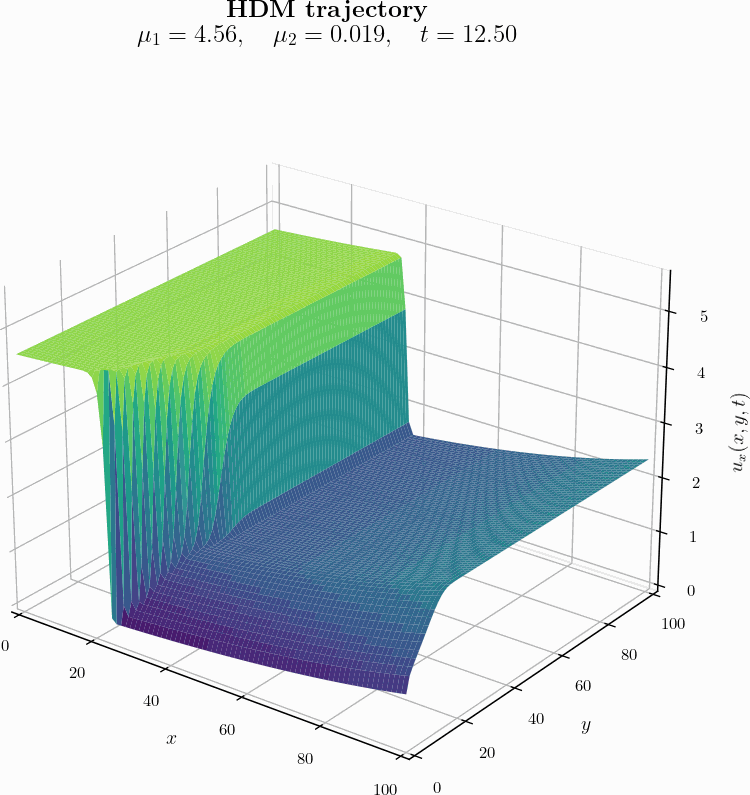
\includegraphics[height=0.56\textheight,keepaspectratio]{Figures/burgers_hdm_3d_transition_cropped.png}\\[0.20cm]
\Large Global and local HPROM validation\\[0.12cm]
\normalsize Linear POD bases, quadratic manifolds, and GPR manifolds
\end{frame}

\begin{frame}{Setup for Paper Campaign}
\small
\textbf{Two-dimensional parametric inviscid Burgers problem}
\[
\frac{\partial \mathbf U}{\partial t}
+\frac{\partial \mathbf F(\mathbf U)}{\partial x}
+\frac{\partial \mathbf G(\mathbf U)}{\partial y}
=\mathbf S(x;\boldsymbol\mu),
\qquad
\mathbf U=
\begin{bmatrix}
u_x\\u_y
\end{bmatrix}.
\]
\[
\mathbf S(x;\boldsymbol\mu)=
\begin{bmatrix}
0.02\exp(\mu_2 x)\\0
\end{bmatrix},
\qquad
u_x(0,y,t;\boldsymbol\mu)=\mu_1.
\]

\vspace{-0.35em}
\centering
\(\mu_1\): inflow value \qquad
\(\mu_2\): exponential source variation \qquad
\(\boldsymbol\mu\in[4.25,5.50]\times[0.015,0.030]\)
\par

\vspace{0.35em}
\textbf{Test points:}
\[
\boldsymbol\mu_1=(4.56,0.019),\quad
\boldsymbol\mu_2=(4.75,0.020),\quad
\boldsymbol\mu_3=(5.19,0.026).
\]

\vspace{-0.25em}
\begin{columns}[T,onlytextwidth]
\begin{column}{0.42\textwidth}
\textbf{HDM:} $\Omega=[0,100]^2$, $250\times250$ finite-volume cells.
\end{column}
\begin{column}{0.58\textwidth}
\textbf{Methods included:}
\begin{tabular}{ll}
Global HPROM & Local HPROM \\
Global HQPROM & Local HQPROM \\
Global HPROM--GPR & Local HPROM--GPR
\end{tabular}
\end{column}
\end{columns}
\end{frame}

\begin{frame}{Parameter Domain and Test Points}
\centering
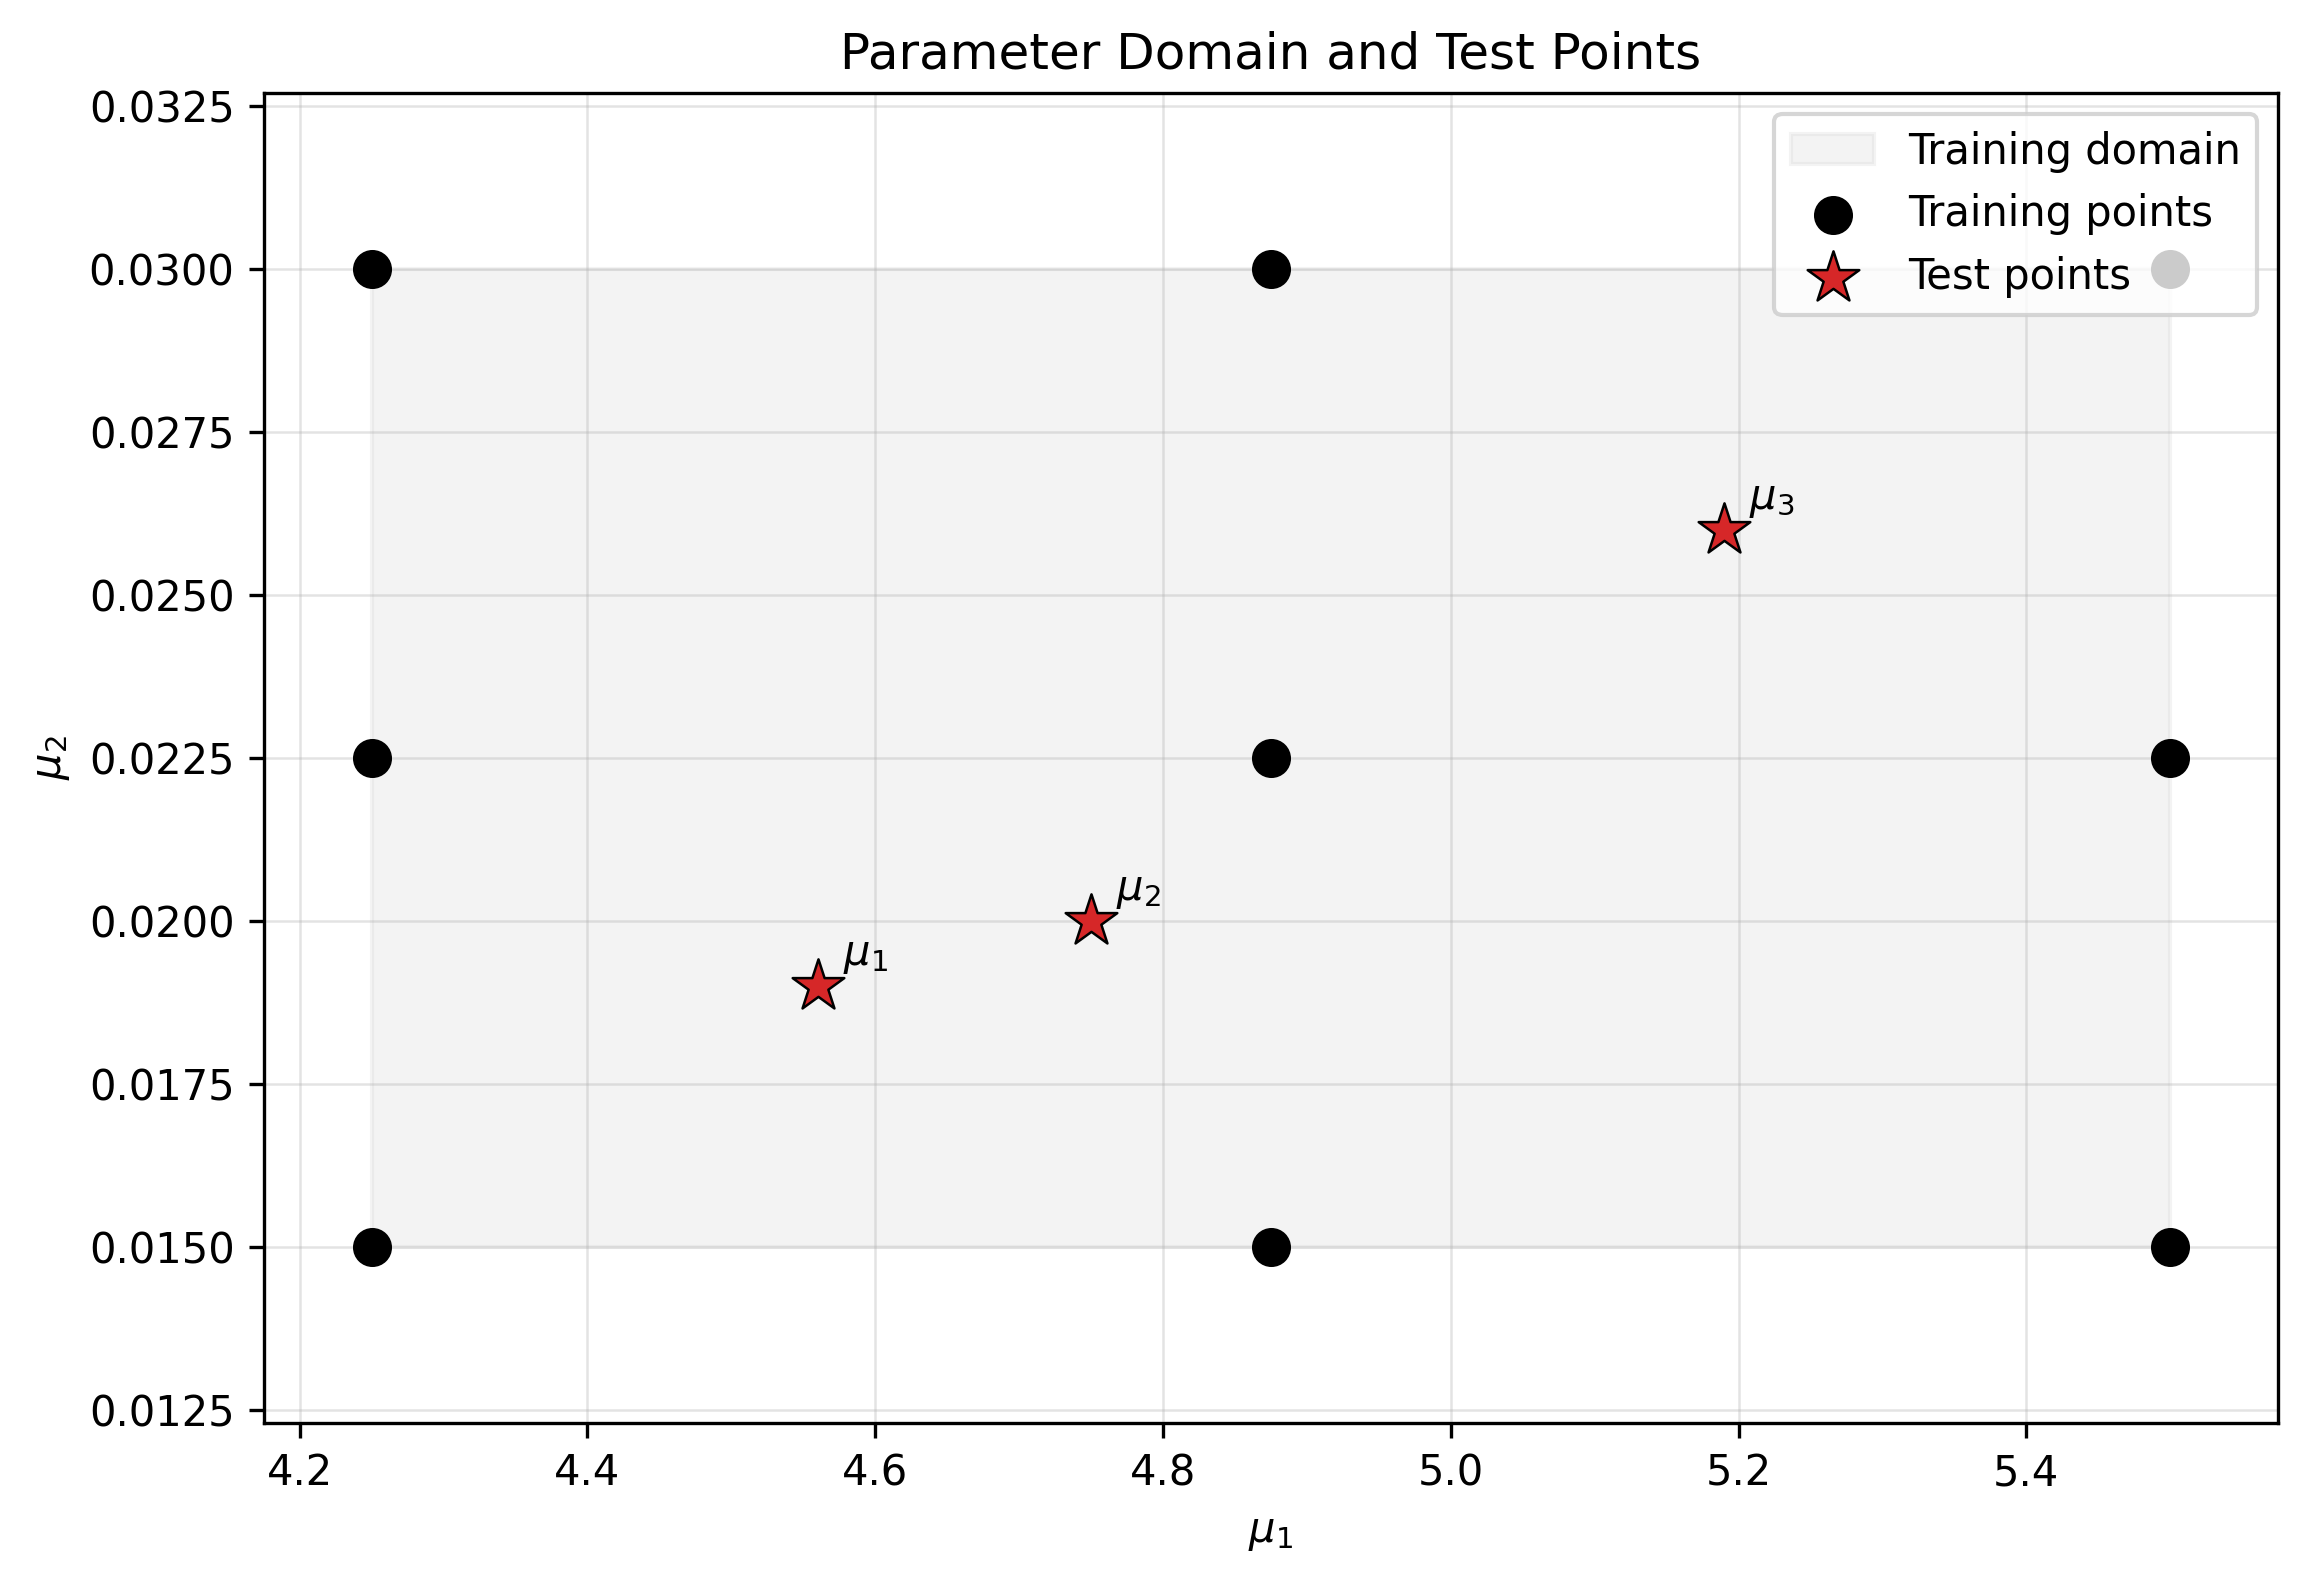
\includegraphics[width=0.82\textwidth,height=0.70\textheight,keepaspectratio]{Figures/parameter_domain_and_test_points.png}
\end{frame}

\newcommand{\BurgersTheoryFrames}{%
\begin{frame}{Global ROM Storyline: LSPG + Gauss-Newton}
\small
Given the implicit HDM residual $\mathbf{r}(\mathbf{u})=\mathbf{0}$, define a manifold
\[
\mathbf{u}\approx \mathbf{u}_{\mathrm{ref}}+\widetilde{\mathbf{u}}(\mathbf{q}).
\]
LSPG solves at each time step:
\[
\mathbf{q}^{\star}
=\arg\min_{\mathbf{q}}\;
\frac{1}{2}\left\|\mathbf{r}\!\left(\mathbf{u}_{\mathrm{ref}}+\widetilde{\mathbf{u}}(\mathbf{q})\right)\right\|_2^2.
\]
With Gauss-Newton (current iterate $\mathbf{q}^{(k)}$), the increment $\Delta\mathbf{q}$ is obtained from
\[
\left(\mathbf{\Psi}^{T}\mathbf{J}^{T}\mathbf{J}\mathbf{\Psi}\right)\Delta\mathbf{q}
=-\mathbf{\Psi}^{T}\mathbf{J}^{T}\mathbf{r},
\]
where
\[
\mathbf{\Psi}=\frac{\partial\widetilde{\mathbf{u}}}{\partial\mathbf{q}},
\qquad
\mathbf{J}=\frac{\partial\mathbf{r}}{\partial\mathbf{u}},
\qquad
\mathbf{q}^{(k+1)}=\mathbf{q}^{(k)}+\Delta\mathbf{q}.
\]
\end{frame}

\begin{frame}{Global Linear HPROM}
\small
State ansatz:
\[
\mathbf{u}\approx \mathbf{u}_{\mathrm{ref}}+\mathbf{V}\mathbf{q},
\qquad
\mathbf{V}\in\mathbb{R}^{N\times n},\; n=96.
\]
Hence
\[
\widetilde{\mathbf{u}}(\mathbf{q})=\mathbf{V}\mathbf{q},
\qquad
\mathbf{\Psi}=\frac{\partial\widetilde{\mathbf{u}}}{\partial\mathbf{q}}=\mathbf{V}.
\]
Gauss-Newton system:
\[
\left(\mathbf{V}^{T}\mathbf{J}^{T}\mathbf{J}\mathbf{V}\right)\Delta\mathbf{q}
=-\mathbf{V}^{T}\mathbf{J}^{T}\mathbf{r}.
\]
\end{frame}

\begin{frame}{Global HQPROM}
\small
Quadratic-manifold ansatz:
\[
\mathbf{u}\approx
\mathbf{u}_{\mathrm{ref}}
+\mathbf{V}\mathbf{q}
+\mathbf{H}\left(\mathbf{q}\otimes\mathbf{q}\right),
\qquad
n=39.
\]
Thus
\[
\widetilde{\mathbf{u}}(\mathbf{q})
=\mathbf{V}\mathbf{q}
+\mathbf{H}\left(\mathbf{q}\otimes\mathbf{q}\right),
\]
and the tangent depends on the current reduced state:
\[
\mathbf{\Psi}(\mathbf{q})
=\frac{\partial\widetilde{\mathbf{u}}}{\partial\mathbf{q}}
=\mathbf{V}
+\frac{\partial}{\partial\mathbf{q}}
\!\left[\mathbf{H}\left(\mathbf{q}\otimes\mathbf{q}\right)\right].
\]
\end{frame}

\begin{frame}{Global HPROM-GPR}
\small
Split basis and reduced coordinates:
\[
\mathbf{V}_{\mathrm{tot}}=[\mathbf{V},\bar{\mathbf{V}}],
\qquad
\mathbf{q}_{\mathrm{tot}}=
\begin{bmatrix}
\mathbf{q}\\
\bar{\mathbf{q}}
\end{bmatrix}.
\]
\[
\bar{\mathbf{q}}=\mathcal{N}_{\mathrm{GPR}}(\mathbf{q}),
\qquad
n=20,\;\bar{n}=131.
\]
State ansatz:
\[
\mathbf{u}\approx
\mathbf{u}_{\mathrm{ref}}
+\widetilde{\mathbf{u}}(\mathbf{q}),
\]
\[
\widetilde{\mathbf{u}}(\mathbf{q})
=\mathbf{V}_{\mathrm{tot}}\mathbf{q}_{\mathrm{tot}}
=\mathbf{V}\mathbf{q}
+\bar{\mathbf{V}}\,\mathcal{N}_{\mathrm{GPR}}(\mathbf{q}).
\]
Effective tangent for Gauss-Newton:
\[
\mathbf{\Psi}(\mathbf{q})
=\frac{\partial\widetilde{\mathbf{u}}}{\partial\mathbf{q}}
=\mathbf{V}
+\bar{\mathbf{V}}\frac{\partial\mathcal{N}_{\mathrm{GPR}}}{\partial\mathbf{q}}.
\]
\end{frame}

\begin{frame}{Local ROMs: Piecewise Manifolds}
\small
Partition the training snapshots into clusters $k=1,\dots,N_c$ and build one local trial manifold per cluster:
\[
\mathbf u \approx \Phi_k(\mathbf q_k).
\]

Examples used in this work:
\[
\Phi_k^{\mathrm{lin}}(\mathbf q)
=
\mathbf u_{0,k}+\mathbf V_k\mathbf q,
\]
\[
\Phi_k^{\mathrm{quad}}(\mathbf q)
=
\mathbf u_{0,k}+\mathbf V_k\mathbf q+\mathbf H_k(\mathbf q\otimes\mathbf q),
\]
\[
\Phi_k^{\mathrm{gpr}}(\mathbf q)
=
\mathbf u_{0,k}+\mathbf V_k\mathbf q+\bar{\mathbf V}_k\,\mathcal N_{\mathrm{GPR},k}(\mathbf q).
\]

\vspace{0.3em}
\textbf{Online workflow}
\begin{enumerate}
\item Select the active cluster.
\item If the cluster changes, transfer the current state to the new local manifold.
\item Solve the local LSPG problem in the active manifold.
\end{enumerate}
\end{frame}

\begin{frame}{Cluster Selection: Final Form (Linear)}
\small
Shared nearest-centroid selector (used in all local models):
\[
k^+=\arg\min_{\ell=1,\dots,N_c}\|\mathbf u^s-\mathbf u_{c,\ell}\|_2^2,
\qquad
\mathbf u^s=\Phi_{k^-}(\mathbf q_{k^-}).
\]

\vspace{0.2em}
For the linear local manifold $\Phi_{k^-}^{\mathrm{lin}}(\mathbf q)=\mathbf u_{0,k^-}+\mathbf V_{k^-}\mathbf q$:
\[
k^+=\arg\min_{\ell=1,\dots,N_c} S_{k^-,\ell}^{\mathrm{lin}}(\mathbf q_{k^-}),
\]
\[
S_{k^-,\ell}^{\mathrm{lin}}(\mathbf q)
=
2\,\mathbf g_{k^-,\ell}^T\mathbf q + d_{k^-,\ell},
\]
with offline-precomputed terms
\[
\mathbf g_{k^-,\ell}
:=
\mathbf V_{k^-}^T(\mathbf u_{0,k^-}-\mathbf u_{c,\ell}),
\qquad
d_{k^-,\ell}
:=
\|\mathbf u_{0,k^-}-\mathbf u_{c,\ell}\|_2^2.
\]
\end{frame}

\begin{frame}{Cluster Selection: Final Form (HQPROM and HPROM-GPR)}
\scriptsize
\textbf{HQPROM selector}
\[
k^+=\arg\min_{\ell} S_{k^-,\ell}^{\mathrm{quad}}(\mathbf q_{k^-}),
\]
\[
S_{k^-,\ell}^{\mathrm{quad}}(\mathbf q)
=
2\,\mathbf g_{k^-,\ell}^T\mathbf q
+
2\,\mathbf m_{k^-,\ell}^T(\mathbf q\otimes\mathbf q)
+
d_{k^-,\ell},
\]
\[
\mathbf m_{k^-,\ell}^T(\mathbf q\otimes\mathbf q)
:=
(\mathbf u_{0,k^-}-\mathbf u_{c,\ell})^T\mathbf H_{k^-}(\mathbf q\otimes\mathbf q).
\]

\vspace{0.35em}
\textbf{HPROM-GPR selector}
\[
k^+=\arg\min_{\ell} S_{k^-,\ell}^{\mathrm{gpr}}(\mathbf q_{k^-}),
\]
\[
S_{k^-,\ell}^{\mathrm{gpr}}(\mathbf q)
=
2\,\mathbf g_{k^-,\ell}^T\mathbf q
+
2\,\bar{\mathbf g}_{k^-,\ell}^T\mathcal N_{\mathrm{GPR},k^-}(\mathbf q)
+
d_{k^-,\ell}.
\]
\[
\bar{\mathbf q}_{k^-}:=\mathcal N_{\mathrm{GPR},k^-}(\mathbf q_{k^-}),
\qquad
\bar{\mathbf g}_{k^-,\ell}:=\bar{\mathbf V}_{k^-}^T(\mathbf u_{0,k^-}-\mathbf u_{c,\ell}).
\]
\end{frame}

\begin{frame}{Cluster Change: Linear and Nonlinear Transfers}
\scriptsize
\[
k^+=k^- \Rightarrow \text{no transfer},
\qquad
k^+\neq k^- \Rightarrow \text{solve transfer problem}.
\]
Transferred state:
\[
\mathbf u^s=\Phi_{k^-}(\mathbf q_{k^-}).
\]

\textbf{Linear local target}
\[
\mathbf q_{k^+}^{\mathrm{lin}}
=\arg\min_{\mathbf q}
\left\|
\mathbf u^s-\left(\mathbf u_{0,k^+}+\mathbf V_{k^+}\mathbf q\right)
\right\|_2^2,
\]
\[
\text{if }\mathbf V_{k^+}^T\mathbf V_{k^+}=\mathbf I,\quad
\mathbf q_{k^+}^{\mathrm{lin}}=\mathbf V_{k^+}^T(\mathbf u^s-\mathbf u_{0,k^+}).
\]

\textbf{Nonlinear local targets (HQPROM / HPROM-GPR)}
\[
\mathbf q_{k^+}^{\mathrm{nl}}
=\arg\min_{\mathbf q}
\left\|\mathbf u^s-\Phi_{k^+}^{\mathrm{nl}}(\mathbf q)\right\|_2^2.
\]
\end{frame}

\begin{frame}{Cluster Change: Nonlinear Least Squares}
\small
For nonlinear local manifolds, define
\[
\mathbf r_{\mathrm{tr}}(\mathbf q):=\Phi_{k^+}(\mathbf q)-\mathbf u^s,
\qquad
\mathbf J_{\Phi}(\mathbf q):=\frac{\partial \Phi_{k^+}}{\partial \mathbf q}.
\]
Gauss--Newton at iterate $\mathbf q^{(j)}$:
\[
\left(\mathbf J_{\Phi}^T\mathbf J_{\Phi}\right)\Delta\mathbf q
=
-\mathbf J_{\Phi}^T\mathbf r_{\mathrm{tr}}(\mathbf q^{(j)}),
\qquad
\mathbf q^{(j+1)}=\mathbf q^{(j)}+\Delta\mathbf q.
\]
\end{frame}

}

\begin{frame}{Online Performance ($250\times250$): Avg/Max Error over 3 Test Points}
\scriptsize
\centering
\resizebox{\textwidth}{!}{%
\begin{tabular}{lrrrrrrr}
\hline
\textbf{Computational model} & $n$ ($N$ for HDM) & $\bar{n}$ & $N_e$ & avg $\mathbb{RE}_{2,\mathbf{u}}$ (\%) & max $\mathbb{RE}_{2,\mathbf{u}}$ (\%) & Wall-clock time (min) & Speedup \\
\hline
HDM & 125\,000 & -- & 62\,500 & -- & -- & 12.512 & -- \\
\addlinespace[0.35em]
HPROM & 96 & -- & 4\,824 & 1.030 & 1.096 & 0.743 & 16.841 \\
HQPROM & 39 & -- & 3\,505 & 0.871 & 0.933 & 0.888 & 14.084 \\
HPROM-GPR & 20 & 131 & 1\,801 & 0.691 & 0.845 & 0.371 & 33.698 \\
\addlinespace[0.35em]
Local HPROM ($N_c=3$) & 35--48 & -- & 3\,649 & 0.827 & 0.854 & 0.377 & 33.168 \\
Local HQPROM ($N_c=3$) & 11--15 & -- & 1\,164 & 0.716 & 0.844 & 0.311 & 40.259 \\
Local HPROM-GPR ($N_c=3$) & 9 & 60--97 & 811 & 0.713 & 0.789 & 0.282 & 44.379 \\
\hline
\end{tabular}}
\vspace{0.2em}

{\tiny Speedup is computed with respect to the HDM runtime, $t_{\mathrm{HDM}}=750.702$ s.}

{\tiny Online timings were measured on Sherlock using one node, 24 MPI ranks, and 24 cores.}

{\tiny $N_e$ denotes the number of sampled ECSW elements ($N_e=62{,}500$ for HDM/full mesh).}

{\tiny Local ROM results shown here use $N_c=3$ clusters; the $N_c=10$ results are reproduced in the appendix.}
\end{frame}

\begin{frame}{Global Reduced Meshes (ECSW)}
\centering
\begin{columns}[T]
\column{0.33\textwidth}
\centering

\includegraphics[width=\linewidth]{hprom_reduced_mesh.png}\\
{\tiny HPROM ($N_e=4{,}824$)}

\column{0.33\textwidth}
\centering

\includegraphics[width=\linewidth]{hqprom_reduced_mesh.png}\\
{\tiny HQPROM ($N_e=3{,}505$)}

\column{0.33\textwidth}
\centering

\includegraphics[width=\linewidth]{hprom_gpr_reduced_mesh.png}\\
{\tiny HPROM-GPR ($N_e=1{,}801$)}
\end{columns}
\end{frame}

\begin{frame}{Local Reduced Meshes (ECSW), $N_c=3$}
\centering
\begin{columns}[T]
\column{0.33\textwidth}
\centering

\includegraphics[width=\linewidth]{local_hprom_reduced_mesh.png}\\
{\tiny Local HPROM ($N_e=3{,}649$)}

\column{0.33\textwidth}
\centering

\includegraphics[width=\linewidth]{local_hqprom_reduced_mesh.png}\\
{\tiny Local HQPROM ($N_e=1{,}164$)}

\column{0.33\textwidth}
\centering

\includegraphics[width=\linewidth]{local_hprom_gpr_reduced_mesh.png}\\
{\tiny Local HPROM-GPR ($N_e=811$)}
\end{columns}
\end{frame}

\begin{frame}{Burgers Conclusions}
\begin{itemize}
  \item All local ROMs improve runtime performance relative to their global counterparts.
  \item Local HPROM--GPR is the fastest model: 0.282 min and 44.379$\times$ speedup.
  \item Its speed comes primarily from the smaller ECSW mesh, with 811 selected elements versus 1,801 for global HPROM--GPR. Local GPR evaluation is also cheaper because the active-cluster regressor is trained with fewer data than the global regressor.
  \item Reported local-model runtimes include cluster selection and any cluster-transfer cost. The decision and transfer rules are formulation-specific and are defined in the appendix.
\end{itemize}
\end{frame}

\newcommand{\BurgersSolutionFigureFrames}{%
\begin{frame}{HPROM vs HDM: $\boldsymbol\mu=(4.56,\,0.019)$}
\centering

\includegraphics[width=0.82\textwidth,height=0.70\textheight,keepaspectratio]{Figures/hprom_vs_hdm_mu1_4.56_mu2_0.019.png}
\end{frame}

\begin{frame}{HPROM vs HDM: $\boldsymbol\mu=(4.75,\,0.020)$}
\centering

\includegraphics[width=0.82\textwidth,height=0.70\textheight,keepaspectratio]{Figures/hprom_vs_hdm_mu1_4.75_mu2_0.020.png}
\end{frame}

\begin{frame}{HPROM vs HDM: $\boldsymbol\mu=(5.19,\,0.026)$}
\centering

\includegraphics[width=0.82\textwidth,height=0.70\textheight,keepaspectratio]{Figures/hprom_vs_hdm_mu1_5.19_mu2_0.026.png}
\end{frame}

\begin{frame}{Local HPROM ($N_c=3$) vs HDM: $\boldsymbol\mu=(4.56,\,0.019)$}
\centering

\includegraphics[width=0.82\textwidth,height=0.70\textheight,keepaspectratio]{Figures/local_hprom_vs_hdm_mu1_4.56_mu2_0.019.png}
\end{frame}

\begin{frame}{Local HPROM ($N_c=3$) vs HDM: $\boldsymbol\mu=(4.75,\,0.020)$}
\centering

\includegraphics[width=0.82\textwidth,height=0.70\textheight,keepaspectratio]{Figures/local_hprom_vs_hdm_mu1_4.75_mu2_0.020.png}
\end{frame}

\begin{frame}{Local HPROM ($N_c=3$) vs HDM: $\boldsymbol\mu=(5.19,\,0.026)$}
\centering

\includegraphics[width=0.82\textwidth,height=0.70\textheight,keepaspectratio]{Figures/local_hprom_vs_hdm_mu1_5.19_mu2_0.026.png}
\end{frame}

\begin{frame}{HQPROM vs HDM: $\boldsymbol\mu=(4.56,\,0.019)$}
\centering

\includegraphics[width=0.82\textwidth,height=0.70\textheight,keepaspectratio]{Figures/hqprom_vs_hdm_mu1_4.56_mu2_0.019.png}
\end{frame}

\begin{frame}{HQPROM vs HDM: $\boldsymbol\mu=(4.75,\,0.020)$}
\centering

\includegraphics[width=0.82\textwidth,height=0.70\textheight,keepaspectratio]{Figures/hqprom_vs_hdm_mu1_4.75_mu2_0.020.png}
\end{frame}

\begin{frame}{HQPROM vs HDM: $\boldsymbol\mu=(5.19,\,0.026)$}
\centering

\includegraphics[width=0.82\textwidth,height=0.70\textheight,keepaspectratio]{Figures/hqprom_vs_hdm_mu1_5.19_mu2_0.026.png}
\end{frame}

\begin{frame}{Local HQPROM ($N_c=3$) vs HDM: $\boldsymbol\mu=(4.56,\,0.019)$}
\centering

\includegraphics[width=0.82\textwidth,height=0.70\textheight,keepaspectratio]{Figures/local_hqprom_vs_hdm_mu1_4.56_mu2_0.019.png}
\end{frame}

\begin{frame}{Local HQPROM ($N_c=3$) vs HDM: $\boldsymbol\mu=(4.75,\,0.020)$}
\centering

\includegraphics[width=0.82\textwidth,height=0.70\textheight,keepaspectratio]{Figures/local_hqprom_vs_hdm_mu1_4.75_mu2_0.020.png}
\end{frame}

\begin{frame}{Local HQPROM ($N_c=3$) vs HDM: $\boldsymbol\mu=(5.19,\,0.026)$}
\centering

\includegraphics[width=0.82\textwidth,height=0.70\textheight,keepaspectratio]{Figures/local_hqprom_vs_hdm_mu1_5.19_mu2_0.026.png}
\end{frame}

\begin{frame}{HPROM-GPR vs HDM: $\boldsymbol\mu=(4.56,\,0.019)$}
\centering

\includegraphics[width=0.82\textwidth,height=0.70\textheight,keepaspectratio]{Figures/hprom_gpr_vs_hdm_mu1_4.56_mu2_0.019.png}
\end{frame}

\begin{frame}{HPROM-GPR vs HDM: $\boldsymbol\mu=(4.75,\,0.020)$}
\centering

\includegraphics[width=0.82\textwidth,height=0.70\textheight,keepaspectratio]{Figures/hprom_gpr_vs_hdm_mu1_4.75_mu2_0.020.png}
\end{frame}

\begin{frame}{HPROM-GPR vs HDM: $\boldsymbol\mu=(5.19,\,0.026)$}
\centering

\includegraphics[width=0.82\textwidth,height=0.70\textheight,keepaspectratio]{Figures/hprom_gpr_vs_hdm_mu1_5.19_mu2_0.026.png}
\end{frame}

\begin{frame}{Local HPROM-GPR ($N_c=3$) vs HDM: $\boldsymbol\mu=(4.56,\,0.019)$}
\centering

\includegraphics[width=0.82\textwidth,height=0.70\textheight,keepaspectratio]{Figures/local_hprom_gpr_vs_hdm_mu1_4.56_mu2_0.019.png}
\end{frame}

\begin{frame}{Local HPROM-GPR ($N_c=3$) vs HDM: $\boldsymbol\mu=(4.75,\,0.020)$}
\centering

\includegraphics[width=0.82\textwidth,height=0.70\textheight,keepaspectratio]{Figures/local_hprom_gpr_vs_hdm_mu1_4.75_mu2_0.020.png}
\end{frame}

\begin{frame}{Local HPROM-GPR ($N_c=3$) vs HDM: $\boldsymbol\mu=(5.19,\,0.026)$}
\centering

\includegraphics[width=0.82\textwidth,height=0.70\textheight,keepaspectratio]{Figures/local_hprom_gpr_vs_hdm_mu1_5.19_mu2_0.026.png}
\end{frame}

}

\section{Hypersonic Vehicle Campaign}

\begin{frame}{Hypersonic Vehicle Campaign}
\centering
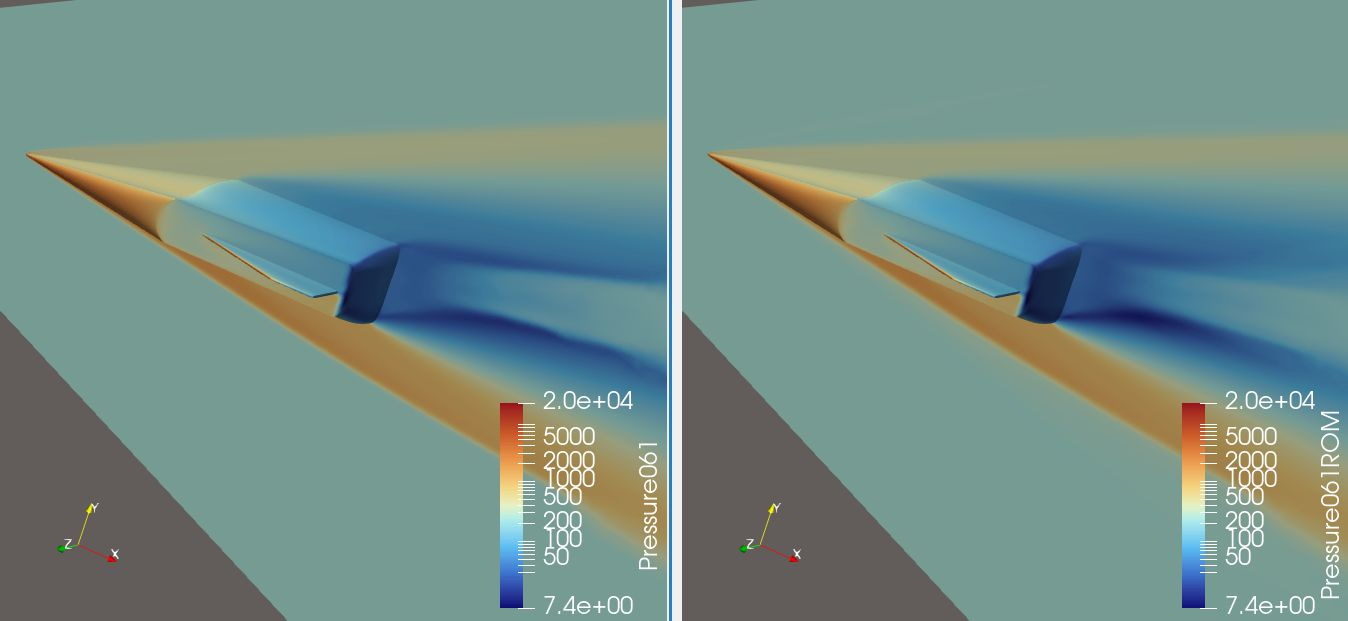
\includegraphics[width=\textwidth,height=0.59\textheight,keepaspectratio]{Figures/img38.jpg}\\[0.25cm]
\Large Global and local HPROM validation\\[0.16cm]
\normalsize Linear POD bases and RBF manifolds
\end{frame}

\begin{frame}{Training and Validation Space}
\centering
\small
363 HDM training cases; 100 independent HDM validation cases; four local clusters with 20\% overlap; ECSW tolerance $10^{-3}$.

\vspace{0.35cm}
\includegraphics[width=0.97\textwidth,height=0.64\textheight,keepaspectratio]{training_validation_space.png}
\end{frame}

\begin{frame}{HGV2 ROM Configurations}
\small
\begin{itemize}
  \item Global linear HPROM uses one POD basis. Local linear HPROM uses four POD bases and assigns each online state to its nearest cluster.
  \item Global HPROM--RBF uses $n=8$ primary coordinates and predicts the remaining coordinates with one RBF map.
  \item Local HPROM--RBF uses one $n=8$ RBF map per cluster. The local primary and secondary dimensions are reported in the next table.
  \item Every POD basis and RBF map is trained from the same 363 HDM parameter cases. ECSW is an independent offline construction step.
\end{itemize}
\end{frame}

\begin{frame}{HGV2 Online Performance and Validation Accuracy}
\centering
\scriptsize
Coefficient errors are global relative $L^2$ values over 100 independent validation cases. Online times are means over 10 validation cases on Sherlock: one node, 24 MPI ranks, and 24 cores.

\vspace{0.12cm}
\renewcommand{\arraystretch}{1.18}
\setlength{\tabcolsep}{2pt}
\resizebox{\textwidth}{!}{%
\begin{tabular}{lccrrrrr}
\toprule
\textbf{Model} & $n$ & $\bar n$ & $C_D$ [\%] & $C_L$ [\%] & $C_M$ [\%] & \textbf{Online time [s]} & \textbf{Speedup} \\
\midrule
Global linear HPROM & 362 & -- & \textbf{0.975} & 0.554 & 6.620 & 24.03 & 1.00 \\
Local linear HPROM, $N_c=4$ & 95--168 & -- & 1.101 & \textbf{0.444} & \textbf{6.242} & 6.80 & 3.53 \\
Global HPROM--RBF & 8 & 354 & 1.388 & 1.335 & 7.004 & 6.00 & 4.00 \\
Local HPROM--RBF, $N_c=4$ & 8 & 117--140 & 1.978 & 2.183 & 7.117 & \textbf{2.28} & \textbf{10.54} \\
\bottomrule
\end{tabular}}

\vspace{0.15cm}
\footnotesize For linear HPROM, $n$ is the full POD rank. For RBF, $n$ and $\bar n$ are the primary and secondary dimensions; local $\bar n$ values are ranges across the four cluster bases. Speedup is relative to global linear HPROM.

\vspace{0.08cm}
\footnotesize Online time is the reported Aero-F nonlinear-ROM timer, including the I/O and postprocessing used to evaluate the $C_L$, $C_D$, and $C_M$ integrals. Fully optimized timings without this I/O remain to be measured.
\end{frame}

\begin{frame}{HGV2 Validation Error Comparison}
\centering
\small The plotted global RBF uses all 363 ECSW parameter cases with row stride 4.

\vspace{0.22cm}
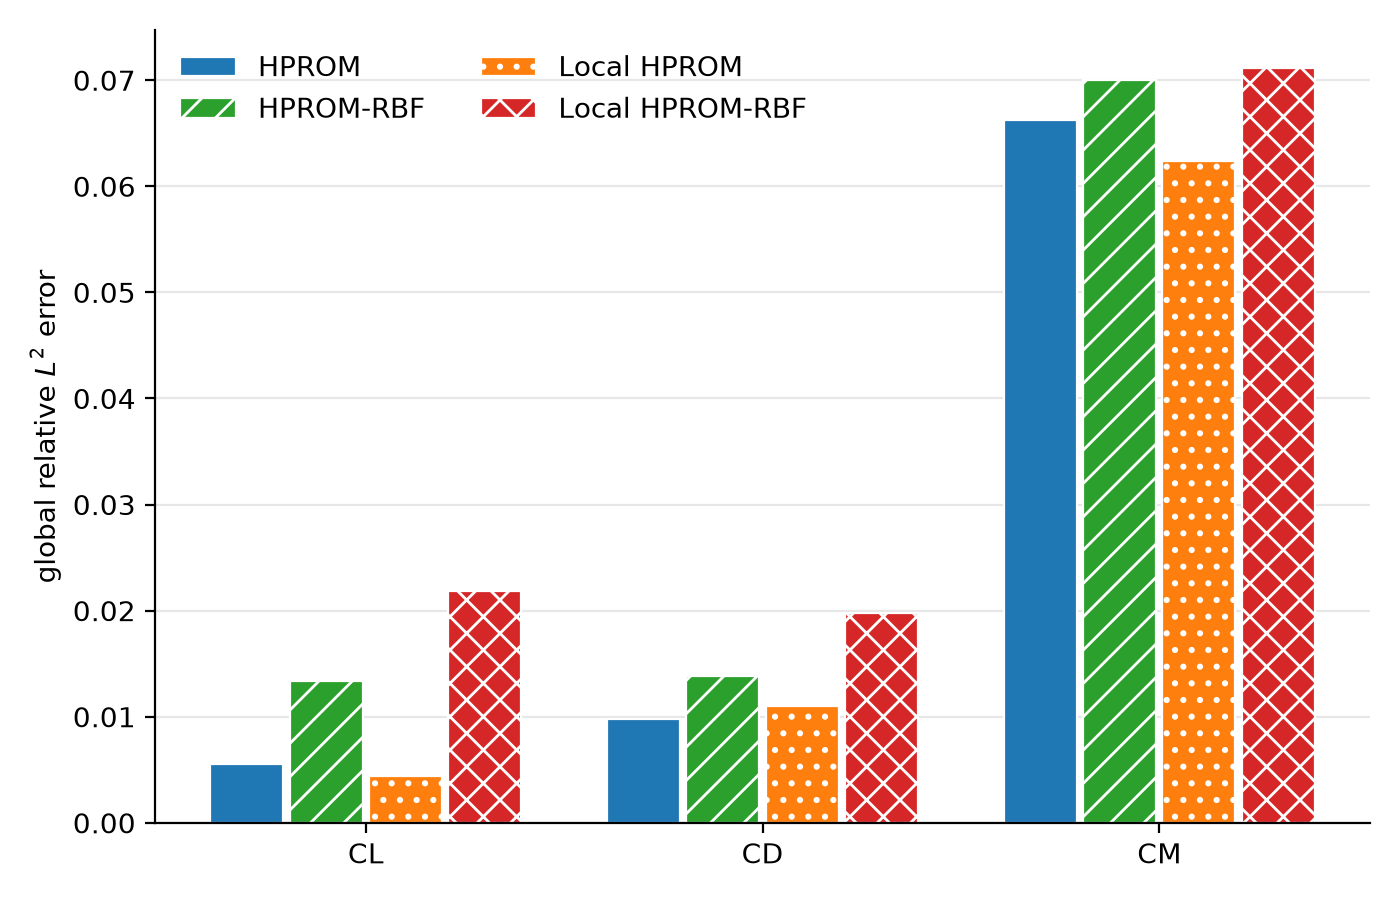
\includegraphics[width=0.91\textwidth,height=0.70\textheight,keepaspectratio]{overall_relative_errors.png}
\end{frame}

\begin{frame}{HGV2 ECSW Offline Cost}
\centering
\scriptsize ECSW was run on Sherlock using 20 nodes, 480 MPI ranks, and 480 cores. Times are maximum-rank wall times from the offline logs.

\vspace{0.12cm}
\renewcommand{\arraystretch}{1.16}
\setlength{\tabcolsep}{2pt}
\resizebox{\textwidth}{!}{%
\begin{tabular}{lrrrrrr}
\toprule
\textbf{Model} & \textbf{Parameter cases} & \textbf{Rows per case} & \textbf{Row stride} & \textbf{Rows read} & \textbf{Sample nodes} & \textbf{ECSW [h]} \\
\midrule
Global linear HPROM & 30 & $30^2$ & 1 & 27,000 & \textbf{5,089} & 30.04 \\
Local linear HPROM, $N_c=4$ & 30 & $30^2$ & 1 & 27,000 & \textbf{3,484} & 9.95 \\
Global HPROM--RBF, $n=8$ & 363 & $8^2$ & 4 & 5,808 & \textbf{1,715} & 0.43 \\
Local HPROM--RBF, $N_c=4$, $n=8$ & 30 & $8^2$ & 1 & 1,920 & \textbf{1,113} & 0.38 \\
\bottomrule
\end{tabular}
}

\vspace{0.14cm}
\begin{block}{What the ECSW columns mean}
\footnotesize Parameter cases $=30$ means a selected subset of the 363 input configurations. For the linear models, $m_k=\min(r_k,30)=30$, hence $30^2$ candidate Jacobian rows per selected case. For RBF, $m_k=n=8$, hence $8^2$ rows. Row stride 4 reads rows $0,4,8,\ldots$ within every one of the 363 global-RBF cases: $363\times8^2/4=5{,}808$ rows. It does not subsample parameter cases or online Newton iterations.
\end{block}
\end{frame}

\begin{frame}{HGV2 Three-Dimensional $C_L$ Error Field}
\centering
\small Each marker is one velocity--altitude pair. Its vertical coordinate is the relative $L^2$ $C_L$ error over the four sampled angles of attack.

\vspace{0.08cm}
\includegraphics[width=0.92\textwidth,height=0.72\textheight,keepaspectratio]{relative_error_3d_CL.png}
\end{frame}

\begin{frame}{HGV2 Two-Dimensional $C_L$ Error Projections}
\centering
\small The front and side projections of the pairwise error field: velocity versus error on the left, altitude versus error on the right.

\vspace{0.08cm}
\includegraphics[width=0.96\textwidth,height=0.72\textheight,keepaspectratio]{relative_error_projections_CL.png}
\end{frame}

\begin{frame}{HGV2 Three-Dimensional $C_D$ Error Field}
\centering
\small Each marker is one velocity--altitude pair. Its vertical coordinate is the relative $L^2$ $C_D$ error over the four sampled angles of attack.

\vspace{0.08cm}
\includegraphics[width=0.92\textwidth,height=0.72\textheight,keepaspectratio]{relative_error_3d_CD.png}
\end{frame}

\begin{frame}{HGV2 Two-Dimensional $C_D$ Error Projections}
\centering
\small The front and side projections of the pairwise error field: velocity versus error on the left, altitude versus error on the right.

\vspace{0.08cm}
\includegraphics[width=0.96\textwidth,height=0.72\textheight,keepaspectratio]{relative_error_projections_CD.png}
\end{frame}

\begin{frame}{HGV2 Three-Dimensional $C_M$ Error Field}
\centering
\small Each marker is one velocity--altitude pair. Its vertical coordinate is the relative $L^2$ $C_M$ error over the four sampled angles of attack.

\vspace{0.08cm}
\includegraphics[width=0.92\textwidth,height=0.72\textheight,keepaspectratio]{relative_error_3d_CM.png}
\end{frame}

\begin{frame}{HGV2 Two-Dimensional $C_M$ Error Projections}
\centering
\small The front and side projections of the pairwise error field: velocity versus error on the left, altitude versus error on the right.

\vspace{0.08cm}
\includegraphics[width=0.96\textwidth,height=0.72\textheight,keepaspectratio]{relative_error_projections_CM.png}
\end{frame}

\begin{frame}{HGV2 Representative Median Pair: $C_L$}
\centering
\small $v=3.495$ km/s, altitude $=59.6$ km. This is the median local-RBF pair after ranking the 25 pairs by the combined $C_L$, $C_D$, and $C_M$ relative-error norm.
\includegraphics[width=0.92\textwidth,height=0.76\textheight,keepaspectratio]{coeff_CL_v3495_alt59600.png}
\end{frame}

\begin{frame}{HGV2 Representative Median Pair: $C_D$}
\centering
\small $v=3.495$ km/s, altitude $=59.6$ km. This is the median local-RBF pair after ranking the 25 pairs by the combined $C_L$, $C_D$, and $C_M$ relative-error norm.
\includegraphics[width=0.92\textwidth,height=0.76\textheight,keepaspectratio]{coeff_CD_v3495_alt59600.png}
\end{frame}

\begin{frame}{HGV2 Representative Median Pair: $C_M$}
\centering
\small $v=3.495$ km/s, altitude $=59.6$ km. This is the median local-RBF pair after ranking the 25 pairs by the combined $C_L$, $C_D$, and $C_M$ relative-error norm.
\includegraphics[width=0.92\textwidth,height=0.76\textheight,keepaspectratio]{coeff_CM_v3495_alt59600.png}
\end{frame}

\begin{frame}{HGV2 Representative Challenging Pair: $C_L$}
\centering
\small $v=3.240$ km/s, altitude $=40.2$ km. This pair has the largest combined local-RBF error across $C_L$, $C_D$, and $C_M$.
\includegraphics[width=0.92\textwidth,height=0.76\textheight,keepaspectratio]{coeff_CL_v3240_alt40200.png}
\end{frame}

\begin{frame}{HGV2 Representative Challenging Pair: $C_D$}
\centering
\small $v=3.240$ km/s, altitude $=40.2$ km. This pair has the largest combined local-RBF error across $C_L$, $C_D$, and $C_M$.
\includegraphics[width=0.92\textwidth,height=0.76\textheight,keepaspectratio]{coeff_CD_v3240_alt40200.png}
\end{frame}

\begin{frame}{HGV2 Representative Challenging Pair: $C_M$}
\centering
\small $v=3.240$ km/s, altitude $=40.2$ km. This pair has the largest combined local-RBF error across $C_L$, $C_D$, and $C_M$.
\includegraphics[width=0.92\textwidth,height=0.76\textheight,keepaspectratio]{coeff_CM_v3240_alt40200.png}
\end{frame}

\begin{frame}{HGV2 Conclusions}
\small
\begin{itemize}
  \item Global and local linear HPROM give the best validation accuracy. Global linear is the best in $C_D$; local linear is the best in $C_L$ and $C_M$.
  \item The global RBF with 363 ECSW cases and row stride 4 is stable and reduces the global-RBF moment error relative to the 30-case, stride-1 ablation, but it does not surpass the linear models.
  \item The local RBF is the fastest online model. Its $C_M$ error is comparable to global RBF, but its $C_L$ and $C_D$ errors are larger. The next controlled test should vary one ECSW factor at a time and broaden the RBF kernel/hyperparameter search.
\end{itemize}
\end{frame}

\appendix

\section{Appendix}

\begin{frame}{Appendix}
\centering
\Large Supplementary results and implementation details
\end{frame}

\section{HGV2 ECSW Details}

\begin{frame}{Appendix: ECSW Training Data}
\centering
\scriptsize
For \texttt{DataType = Jacobian}, each selected parameter solution assigned to cluster $k$ supplies
$m_k^2$ candidate ECSW rows, where
$m_k=\min\!\left(r_k,\ \texttt{MaxNumResidualComponents}\right)$ and
\texttt{MaxNumResidualComponents} $=30$. With row stride $s$, CM reads every $s$-th row of its \texttt{training\_rows} sequence.

\vspace{0.08cm}
\renewcommand{\arraystretch}{1.10}
\setlength{\tabcolsep}{3pt}
\resizebox{0.98\textwidth}{!}{%
\begin{tabular}{lcccc}
\toprule
\textbf{Model} & \textbf{ECSW cases} & \textbf{Row stride} & $m_k$ & \textbf{Rows read by CM} \\
\midrule
Global linear HPROM & 30 & 1 & $\min(362,30)=30$ & $30\times30^2=27{,}000$ \\
Local linear HPROM, $N_c=4$ & 30 & 1 & $\min(r_k,30)=30$ & $30\times30^2=27{,}000$ \\
Global HPROM--RBF, $n=8$ (ablation) & 30 & 1 & $\min(8,30)=8$ & $30\times8^2=1{,}920$ \\
Global HPROM--RBF, $n=8$ (final) & 363 & 4 & $\min(8,30)=8$ & $363\times8^2/4=5{,}808$ \\
Local HPROM--RBF, $N_c=4$, $n=8$ & 30 & 1 & $\min(8,30)=8$ & $30\times8^2=1{,}920$ \\
\bottomrule
\end{tabular}
}

\vspace{0.08cm}
\begin{block}{Interpretation}
\tiny An ECSW snapshot is a Jacobian-training row, not a physical-time state. The RBF primary dimension $n=8$---not $\bar n$---sets the $8\times8$ count. A row stride of 4 reads rows $0,4,8,\ldots$ within every selected parameter case; it does not subsample the 363 parameter cases and does not refer to online Newton iterations.
\end{block}
\end{frame}

\begin{frame}{Appendix: HGV2 Reduced-Mesh Construction}
\centering
\scriptsize
\renewcommand{\arraystretch}{1.17}
\setlength{\tabcolsep}{2pt}
\begin{tabular}{lrrrrrrr}
\toprule
Model & L0 & L1 & L2 & L3 & Nodes & Elems. & $N_{\neg L2}$ \\
\midrule
Global linear HPROM & 5,089 & 36,971 & 166,878 & 60,623 & 269,561 & 563,301 & 92,683 \\
Local linear HPROM, 4 clusters & 3,484 & 28,145 & 169,798 & 47,183 & 248,610 & 470,649 & 78,812 \\
Global HPROM--RBF, $n=8$ & 1,715 & 15,809 & 173,072 & 28,648 & 219,244 & 350,921 & 46,172 \\
Local HPROM--RBF, 4 clusters, $n=8$ & 1,113 & 10,516 & 175,813 & 20,602 & 208,044 & 298,219 & 32,231 \\
\bottomrule
\end{tabular}

\vspace{0.32cm}
\begin{columns}[T,onlytextwidth]
\begin{column}{0.50\textwidth}
\textbf{L0}: selected ECSW sample nodes.\\
\textbf{L1}: nodes added by edge connectivity for linear reconstruction.
\end{column}
\begin{column}{0.50\textwidth}
\textbf{L2}: lift-surface nodes used only for $C_L$, $C_D$, and $C_M$ postprocessing.\\
\textbf{L3}: nodes added by element connectivity for state reconstruction.
\end{column}
\end{columns}

\vspace{0.18cm}
\footnotesize $N_{\neg L2}$ excludes the postprocessing-only lift-surface nodes.
\end{frame}

\section{Theory}
\BurgersTheoryFrames

\section{Burgers Solution Comparisons}
\BurgersSolutionFigureFrames

\section{Burgers $N_c=10$}

\begin{frame}{Appendix: Local ROM Results at $N_c=10$}
\scriptsize
\centering
\resizebox{\textwidth}{!}{%
\begin{tabular}{lrrrrrrr}
\hline
\textbf{Computational model} & $n$ & $\bar{n}$ & $N_e$ & avg $\mathbb{RE}_{2,\mathbf{u}}$ (\%) & max $\mathbb{RE}_{2,\mathbf{u}}$ (\%) & Wall-clock time (min) & Speedup \\
\hline
Local HPROM ($N_c=10$) & 14--23 & -- & 1\,522 & 0.867 & 0.956 & 0.198 & 63.257 \\
Local HQPROM ($N_c=10$) & 8--12 & -- & 871 & 0.572 & 0.929 & 0.263 & 47.497 \\
Local HPROM-GPR ($N_c=10$) & 6 & 24--47 & 541 & 0.604 & 0.801 & 0.244 & 51.261 \\
\hline
\end{tabular}}
\vspace{0.2em}

{\tiny Speedup is computed with respect to the HDM runtime, $t_{\mathrm{HDM}}=750.702$ s.}

{\tiny Global-model rows are unaffected by $N_c$ and are reproduced in the main results table.}
\end{frame}

\begin{frame}{Appendix: Local Reduced Meshes (ECSW), $N_c=10$}
\centering
\begin{columns}[T]
\column{0.33\textwidth}
\centering
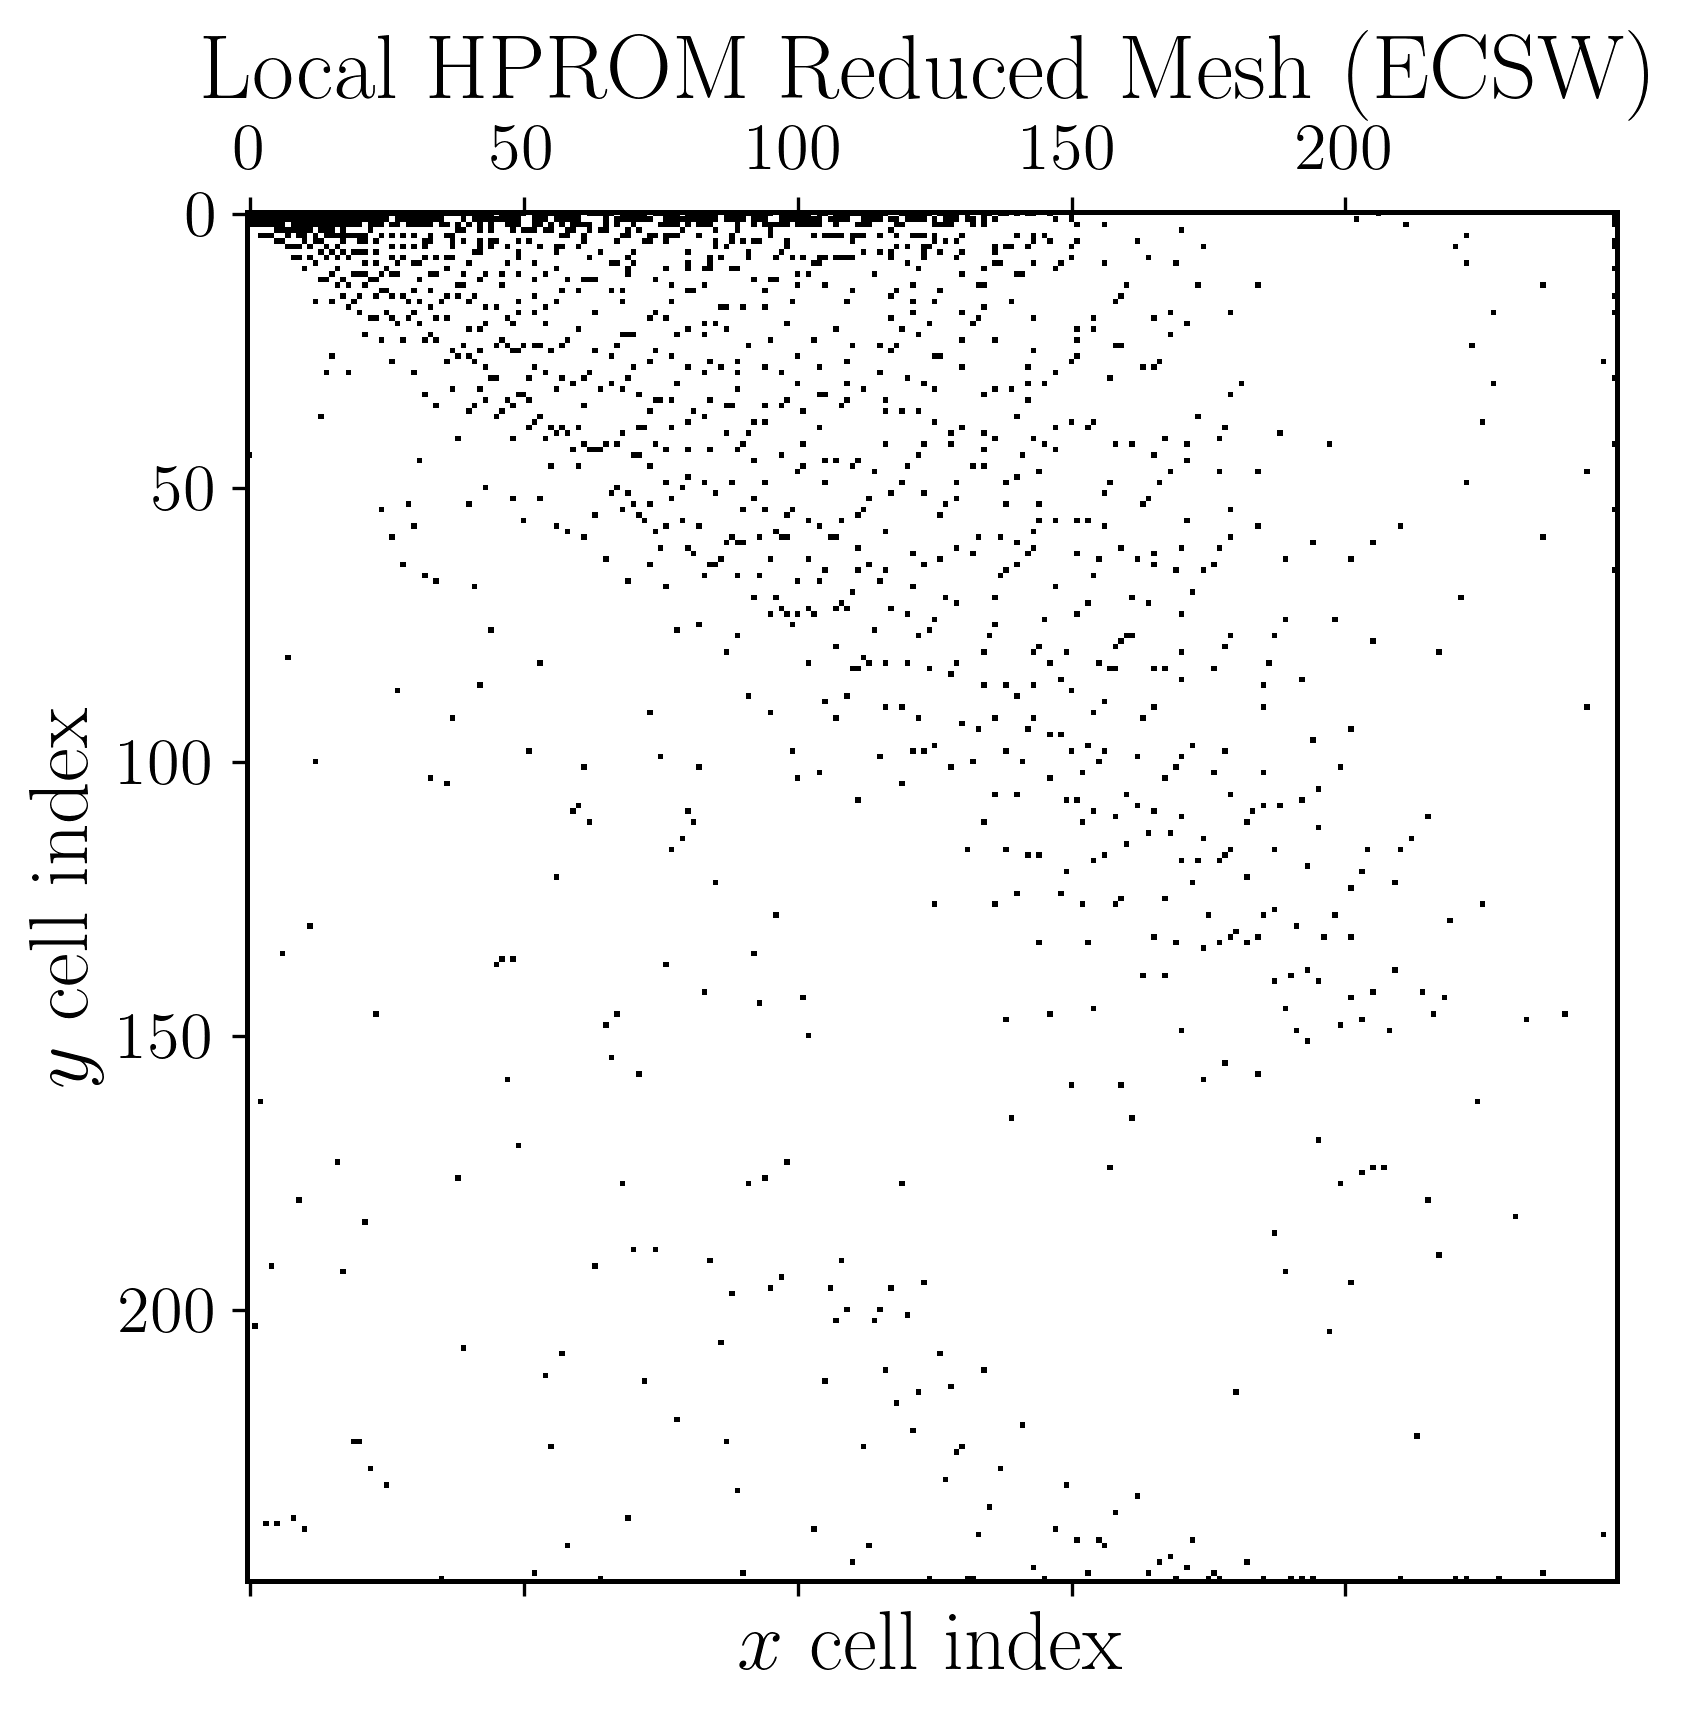
\includegraphics[width=\linewidth]{local_hprom_reduced_mesh_nc10.png}\\
{\tiny Local HPROM ($N_e=1{,}522$)}

\column{0.33\textwidth}
\centering
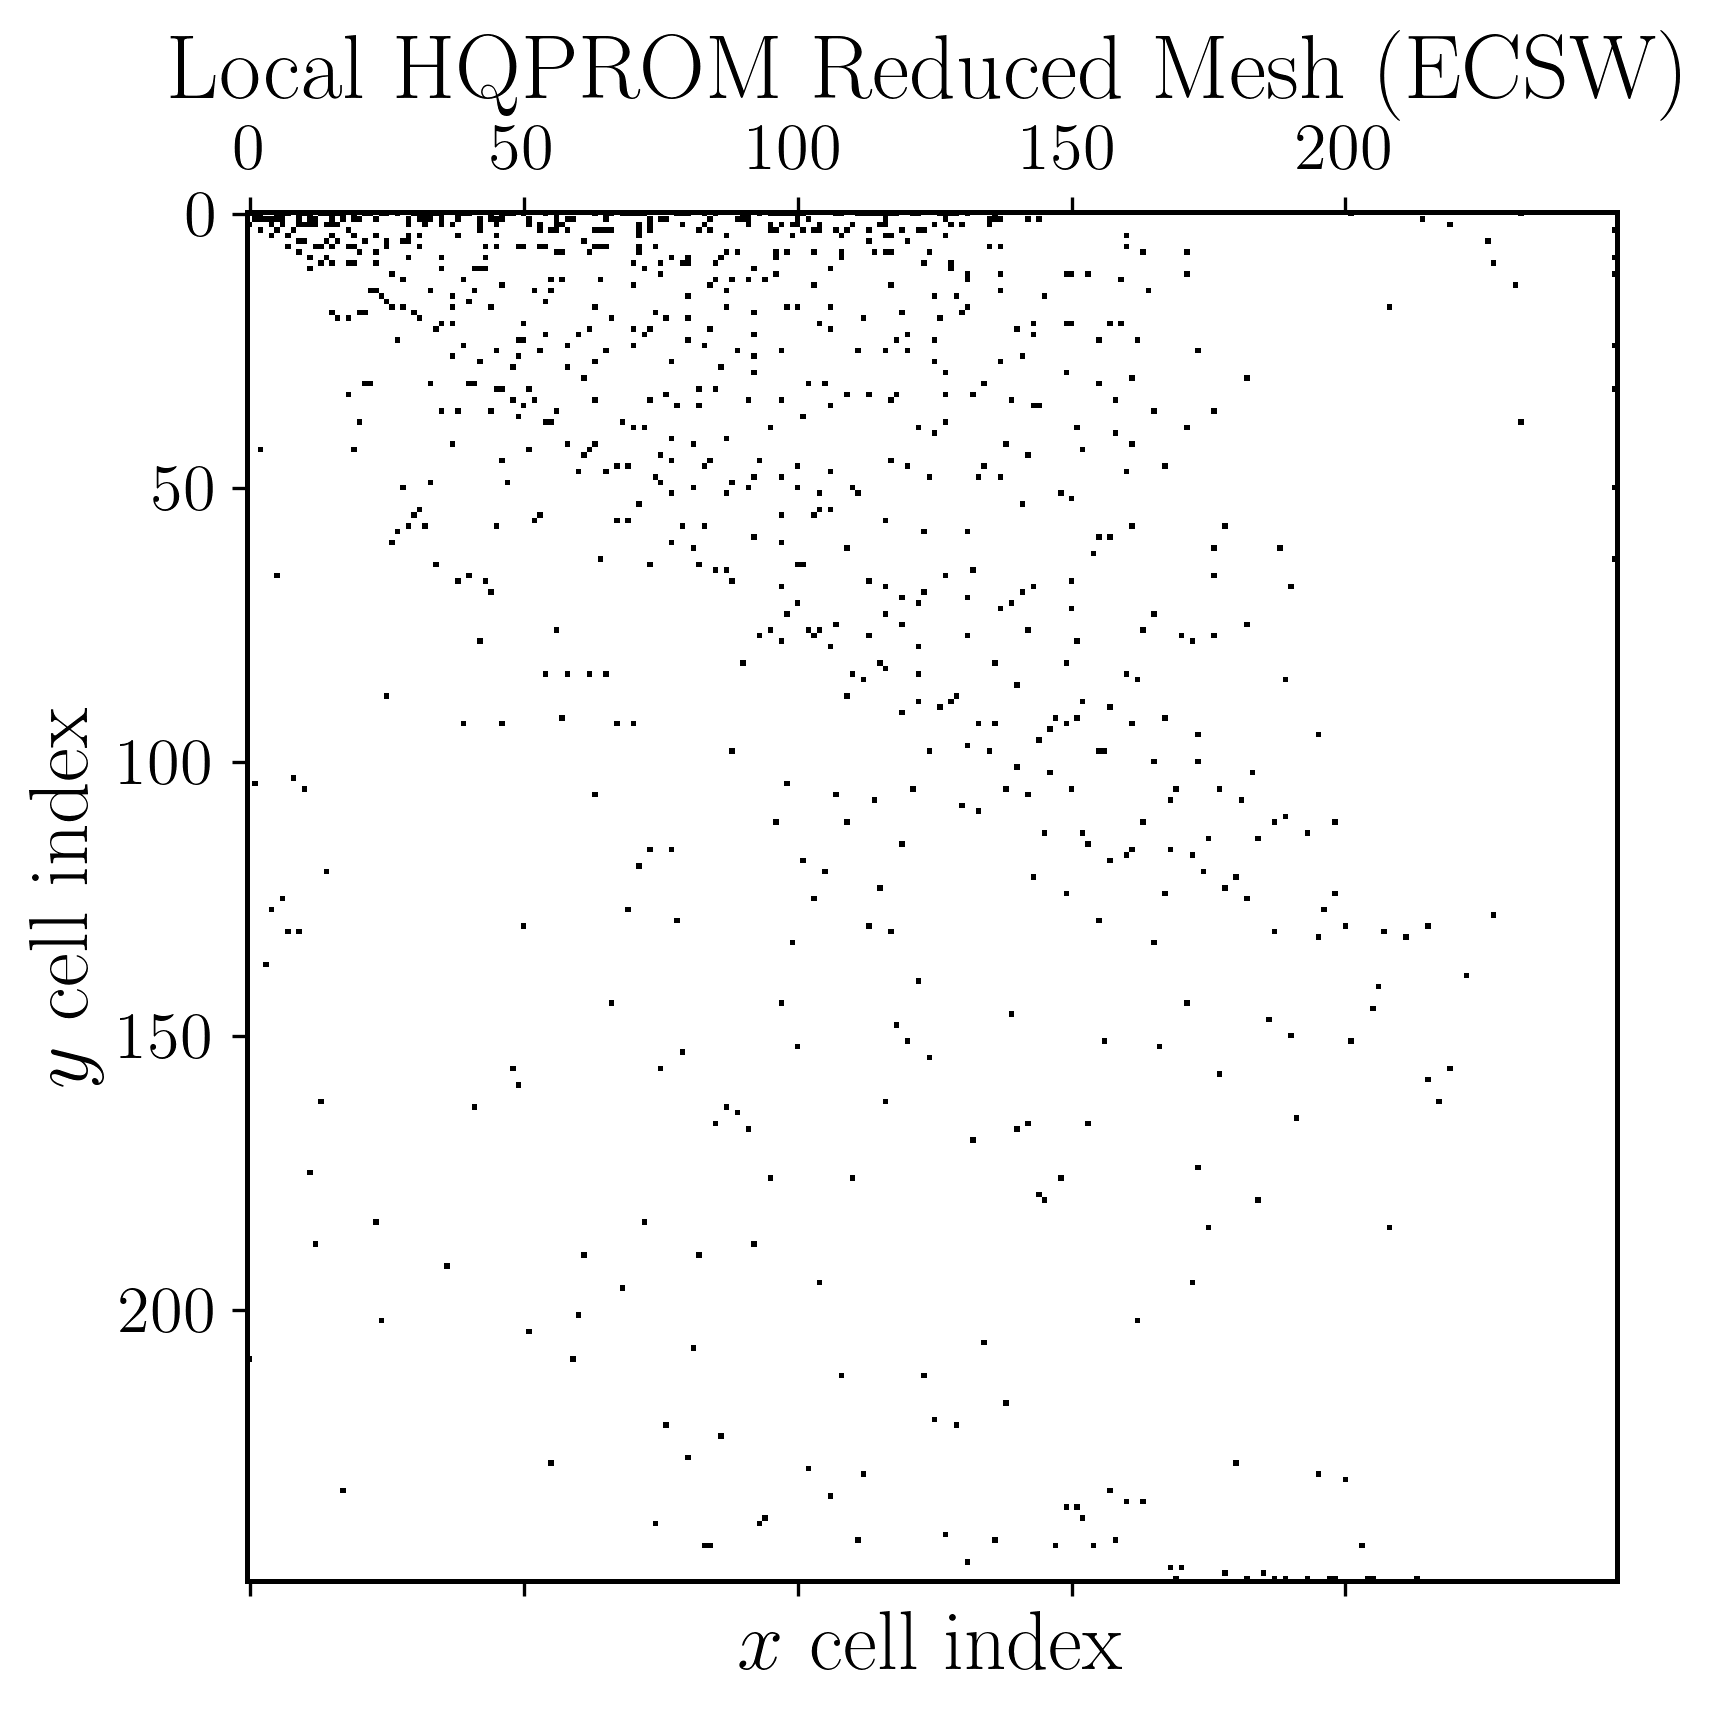
\includegraphics[width=\linewidth]{local_hqprom_reduced_mesh_nc10.png}\\
{\tiny Local HQPROM ($N_e=871$)}

\column{0.33\textwidth}
\centering
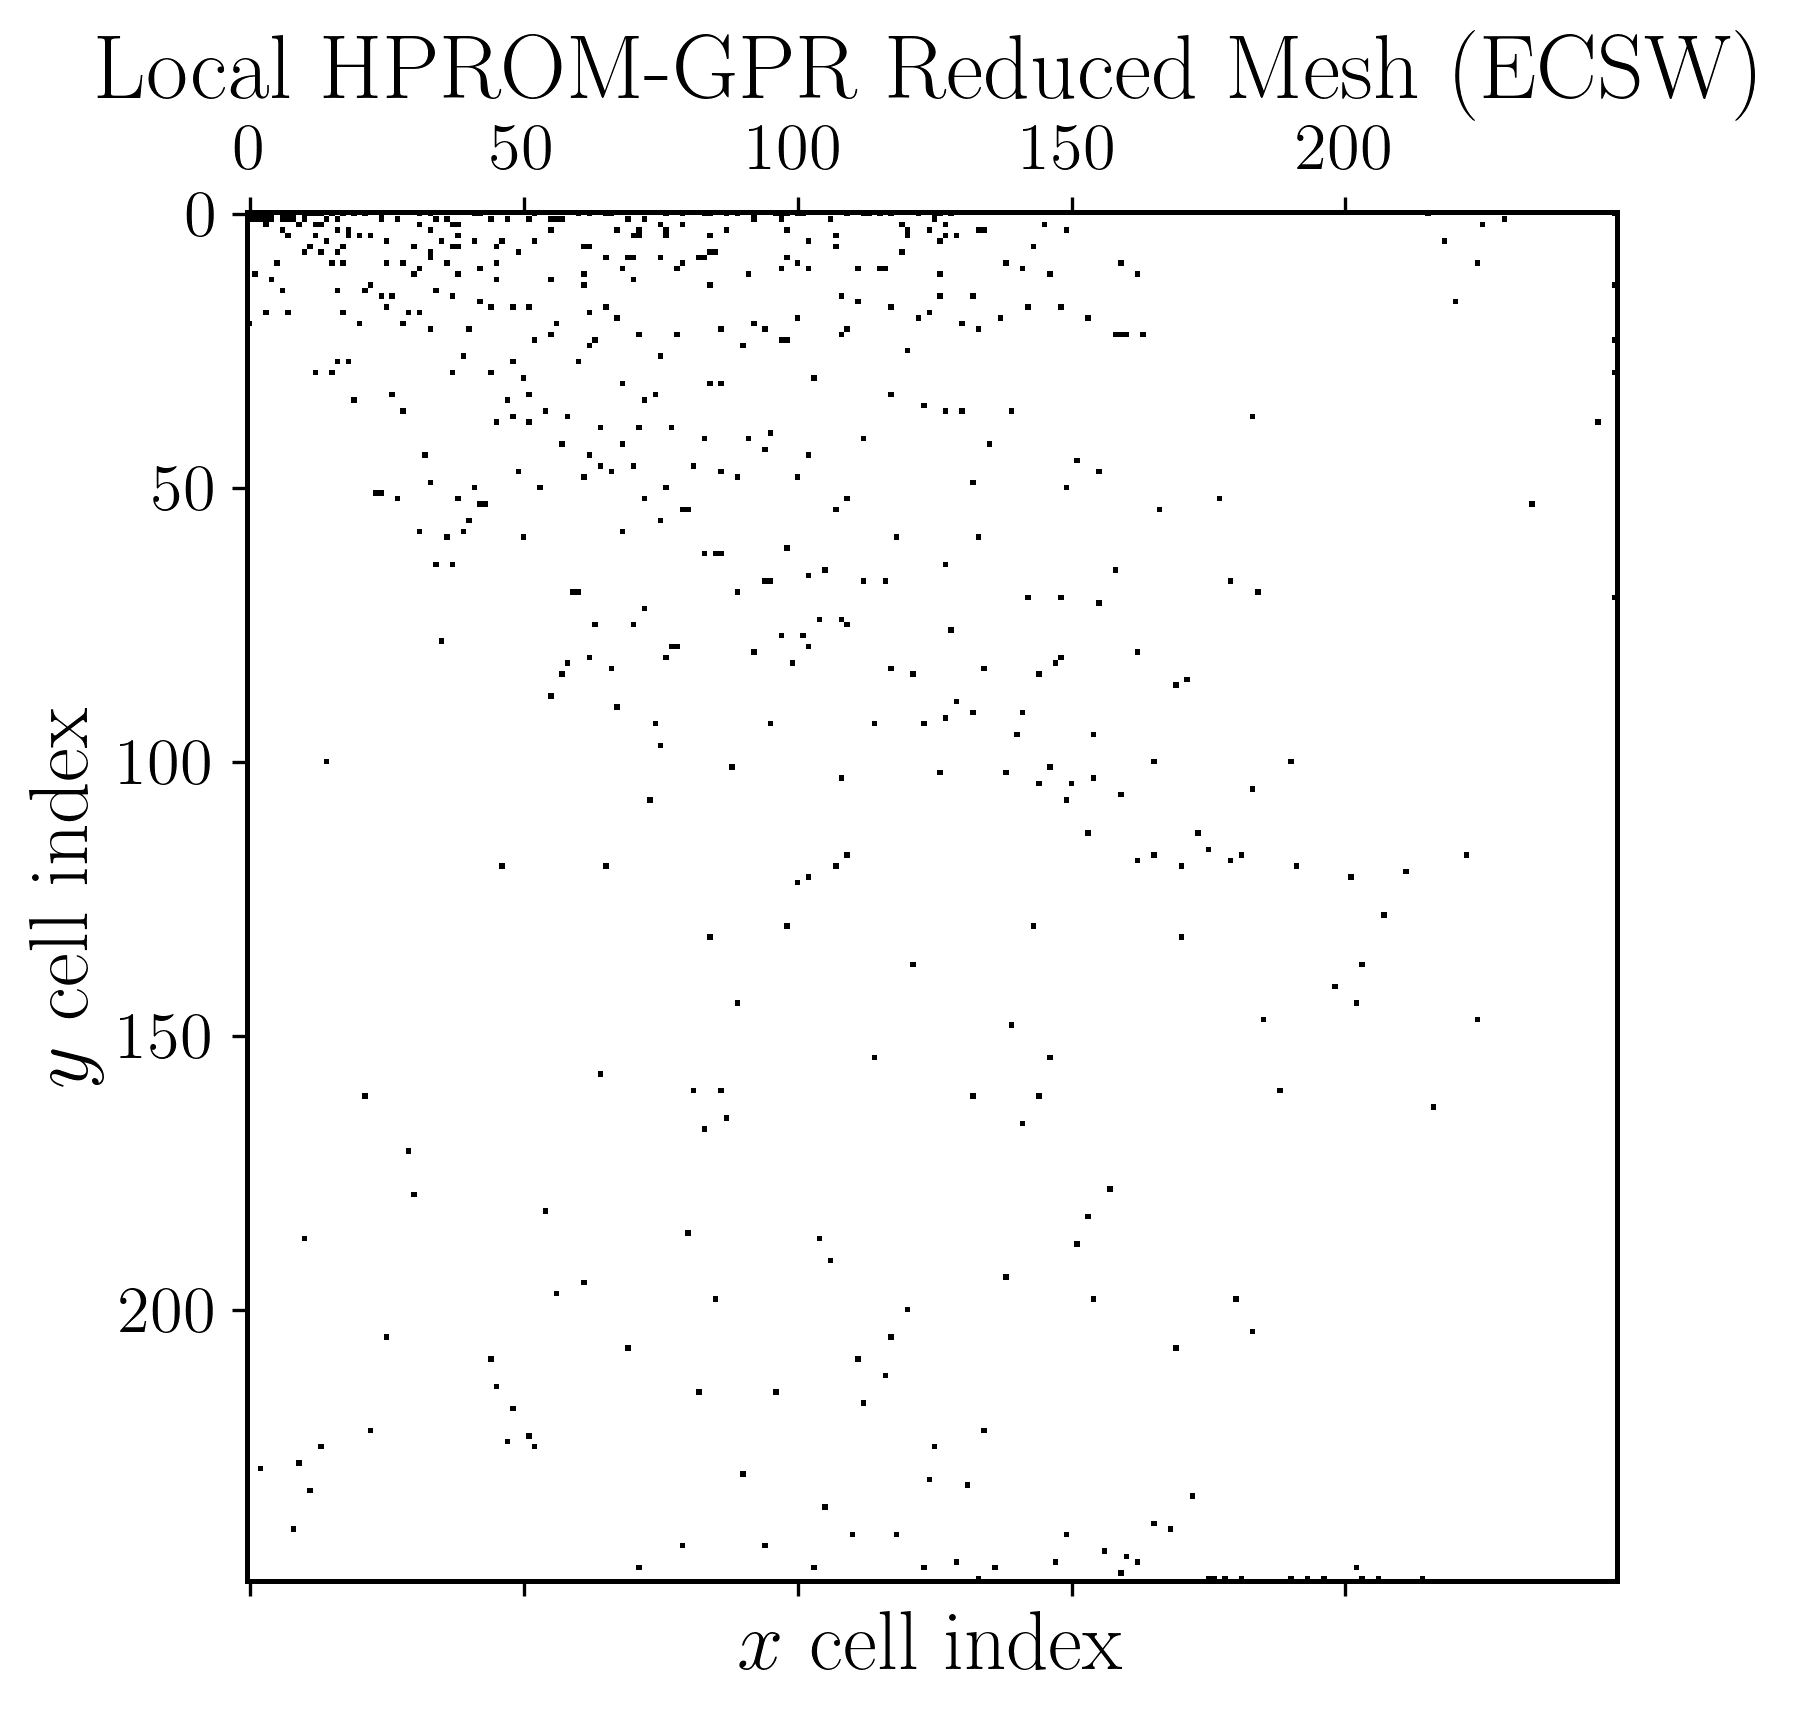
\includegraphics[width=\linewidth]{local_hprom_gpr_reduced_mesh_nc10.png}\\
{\tiny Local HPROM-GPR ($N_e=541$)}
\end{columns}
\end{frame}

\begin{frame}{Appendix: Local HPROM ($N_c=10$) vs HDM: $\boldsymbol\mu=(4.56,\,0.019)$}
\centering
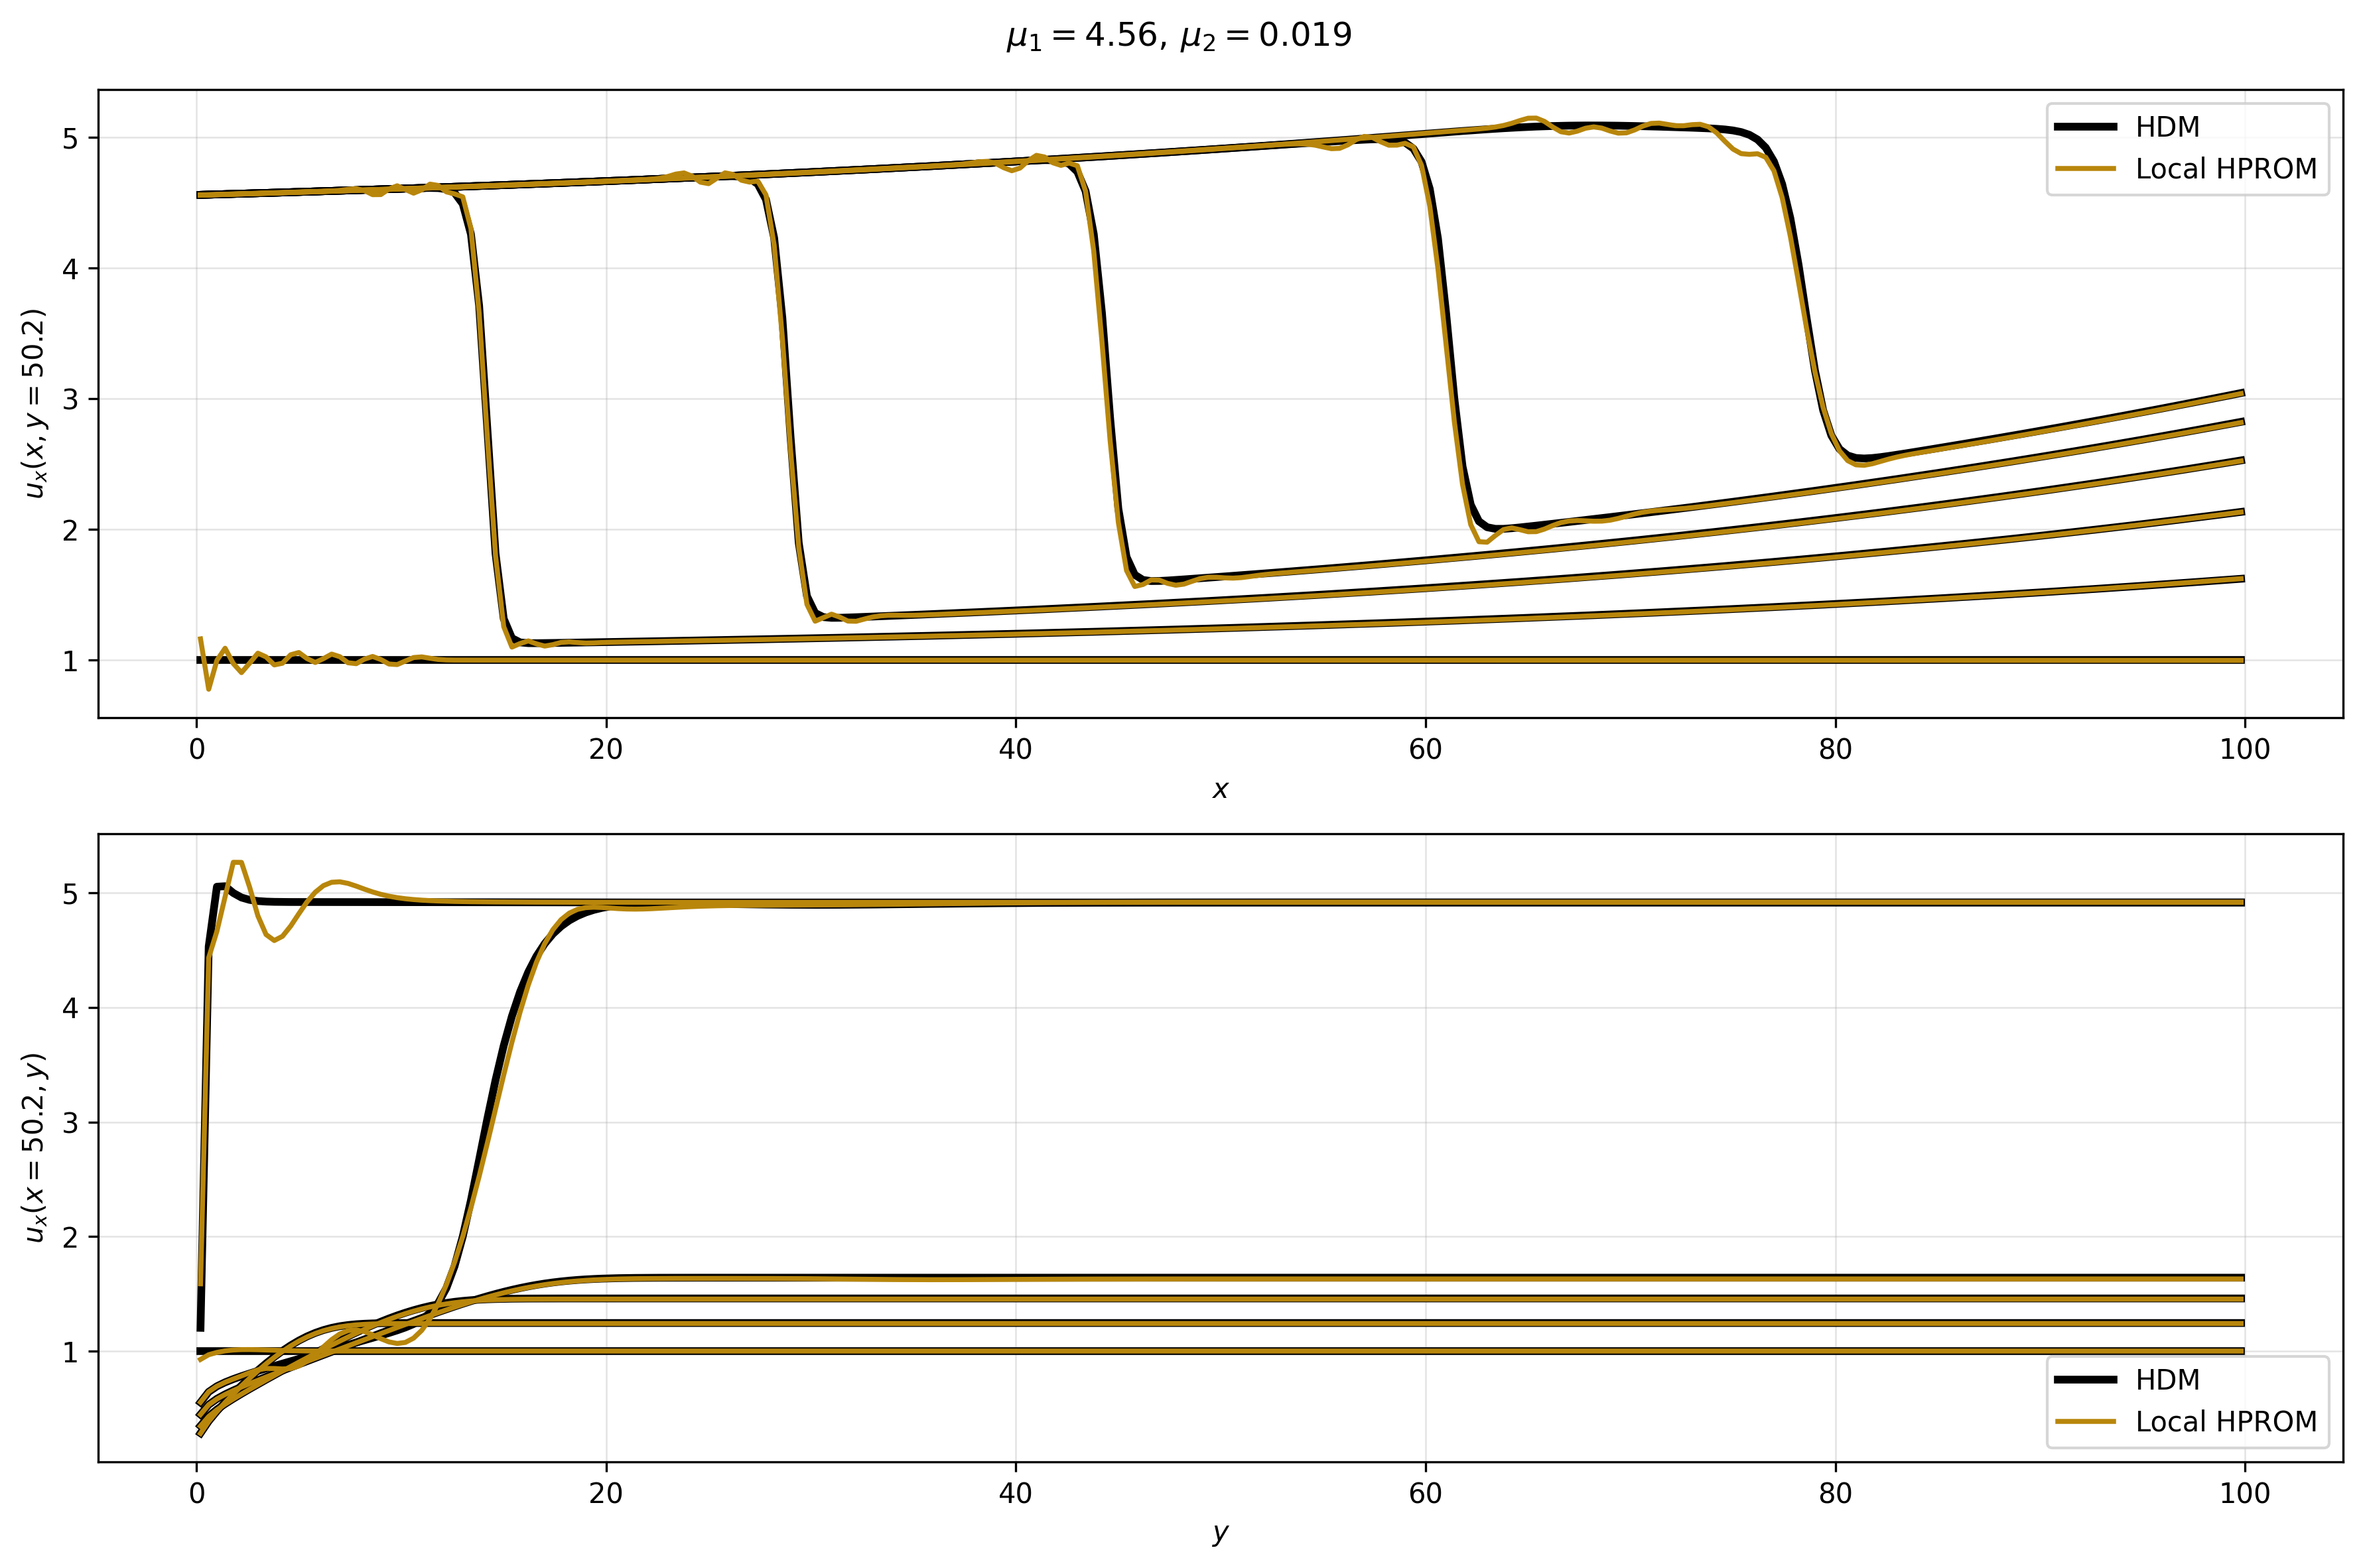
\includegraphics[width=0.82\textwidth,height=0.70\textheight,keepaspectratio]{Figures/local_hprom_vs_hdm_mu1_4.56_mu2_0.019_nc10.png}
\end{frame}

\begin{frame}{Appendix: Local HPROM ($N_c=10$) vs HDM: $\boldsymbol\mu=(4.75,\,0.020)$}
\centering
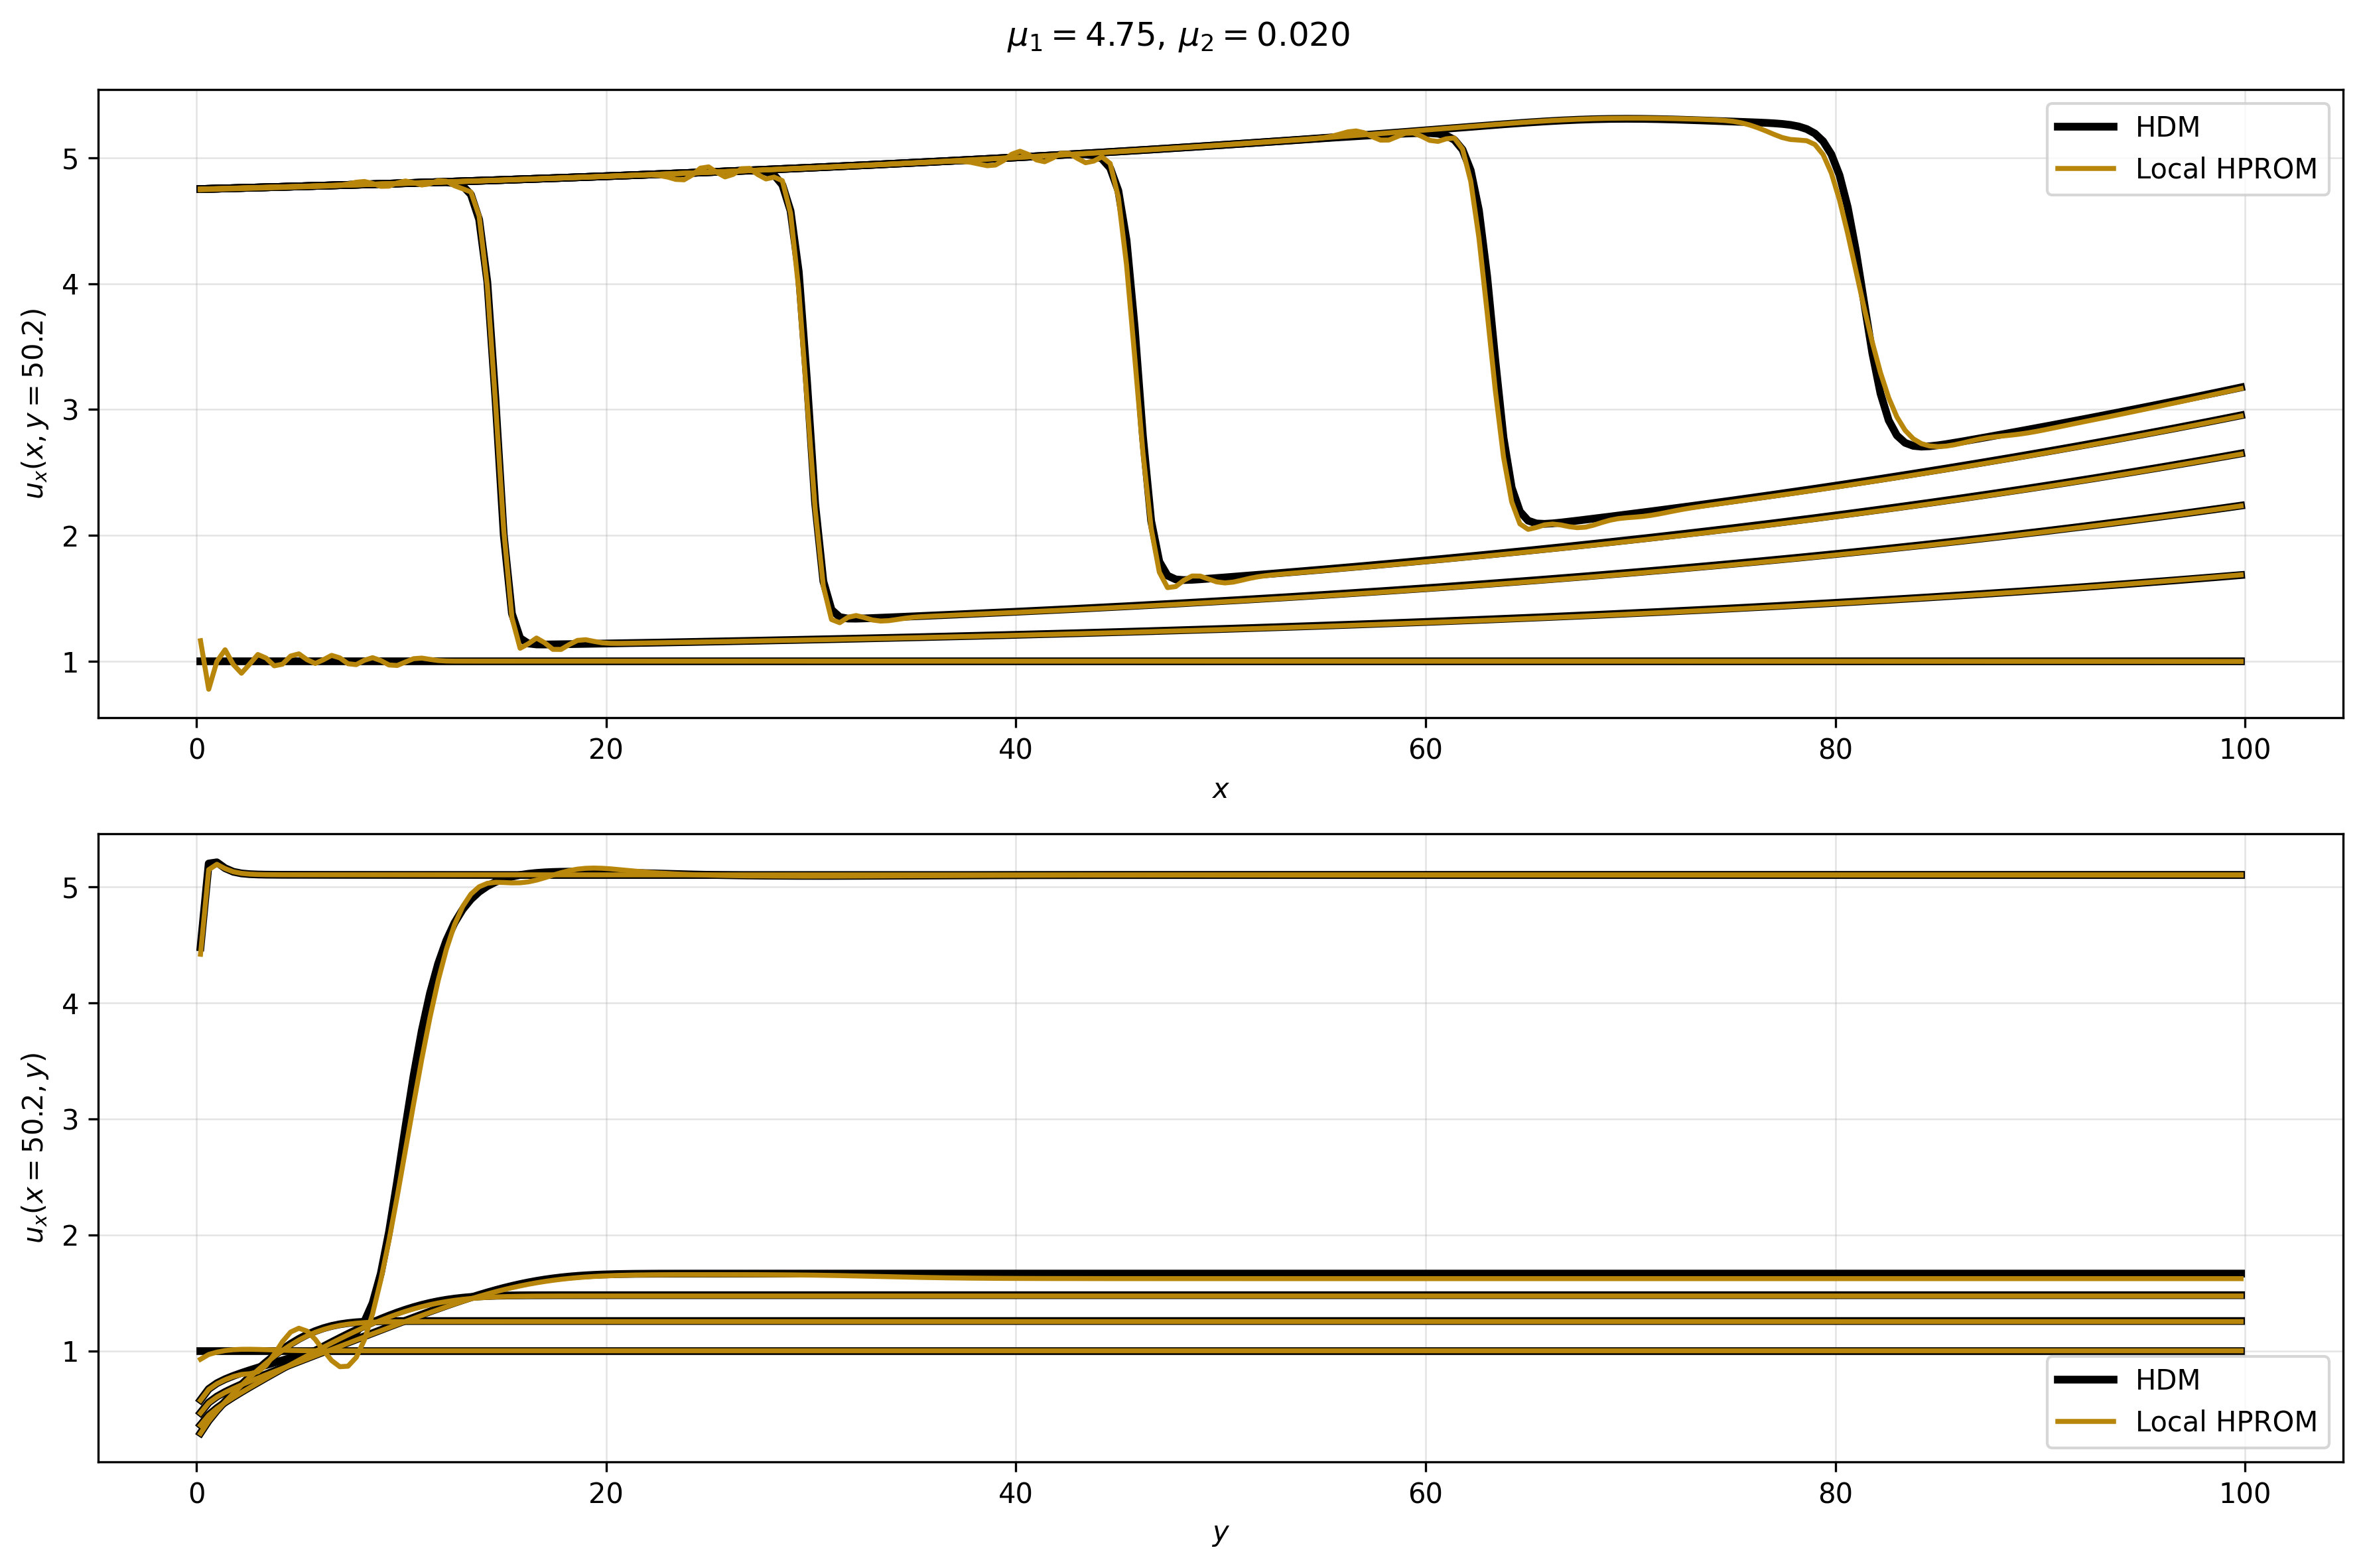
\includegraphics[width=0.82\textwidth,height=0.70\textheight,keepaspectratio]{Figures/local_hprom_vs_hdm_mu1_4.75_mu2_0.020_nc10.png}
\end{frame}

\begin{frame}{Appendix: Local HPROM ($N_c=10$) vs HDM: $\boldsymbol\mu=(5.19,\,0.026)$}
\centering
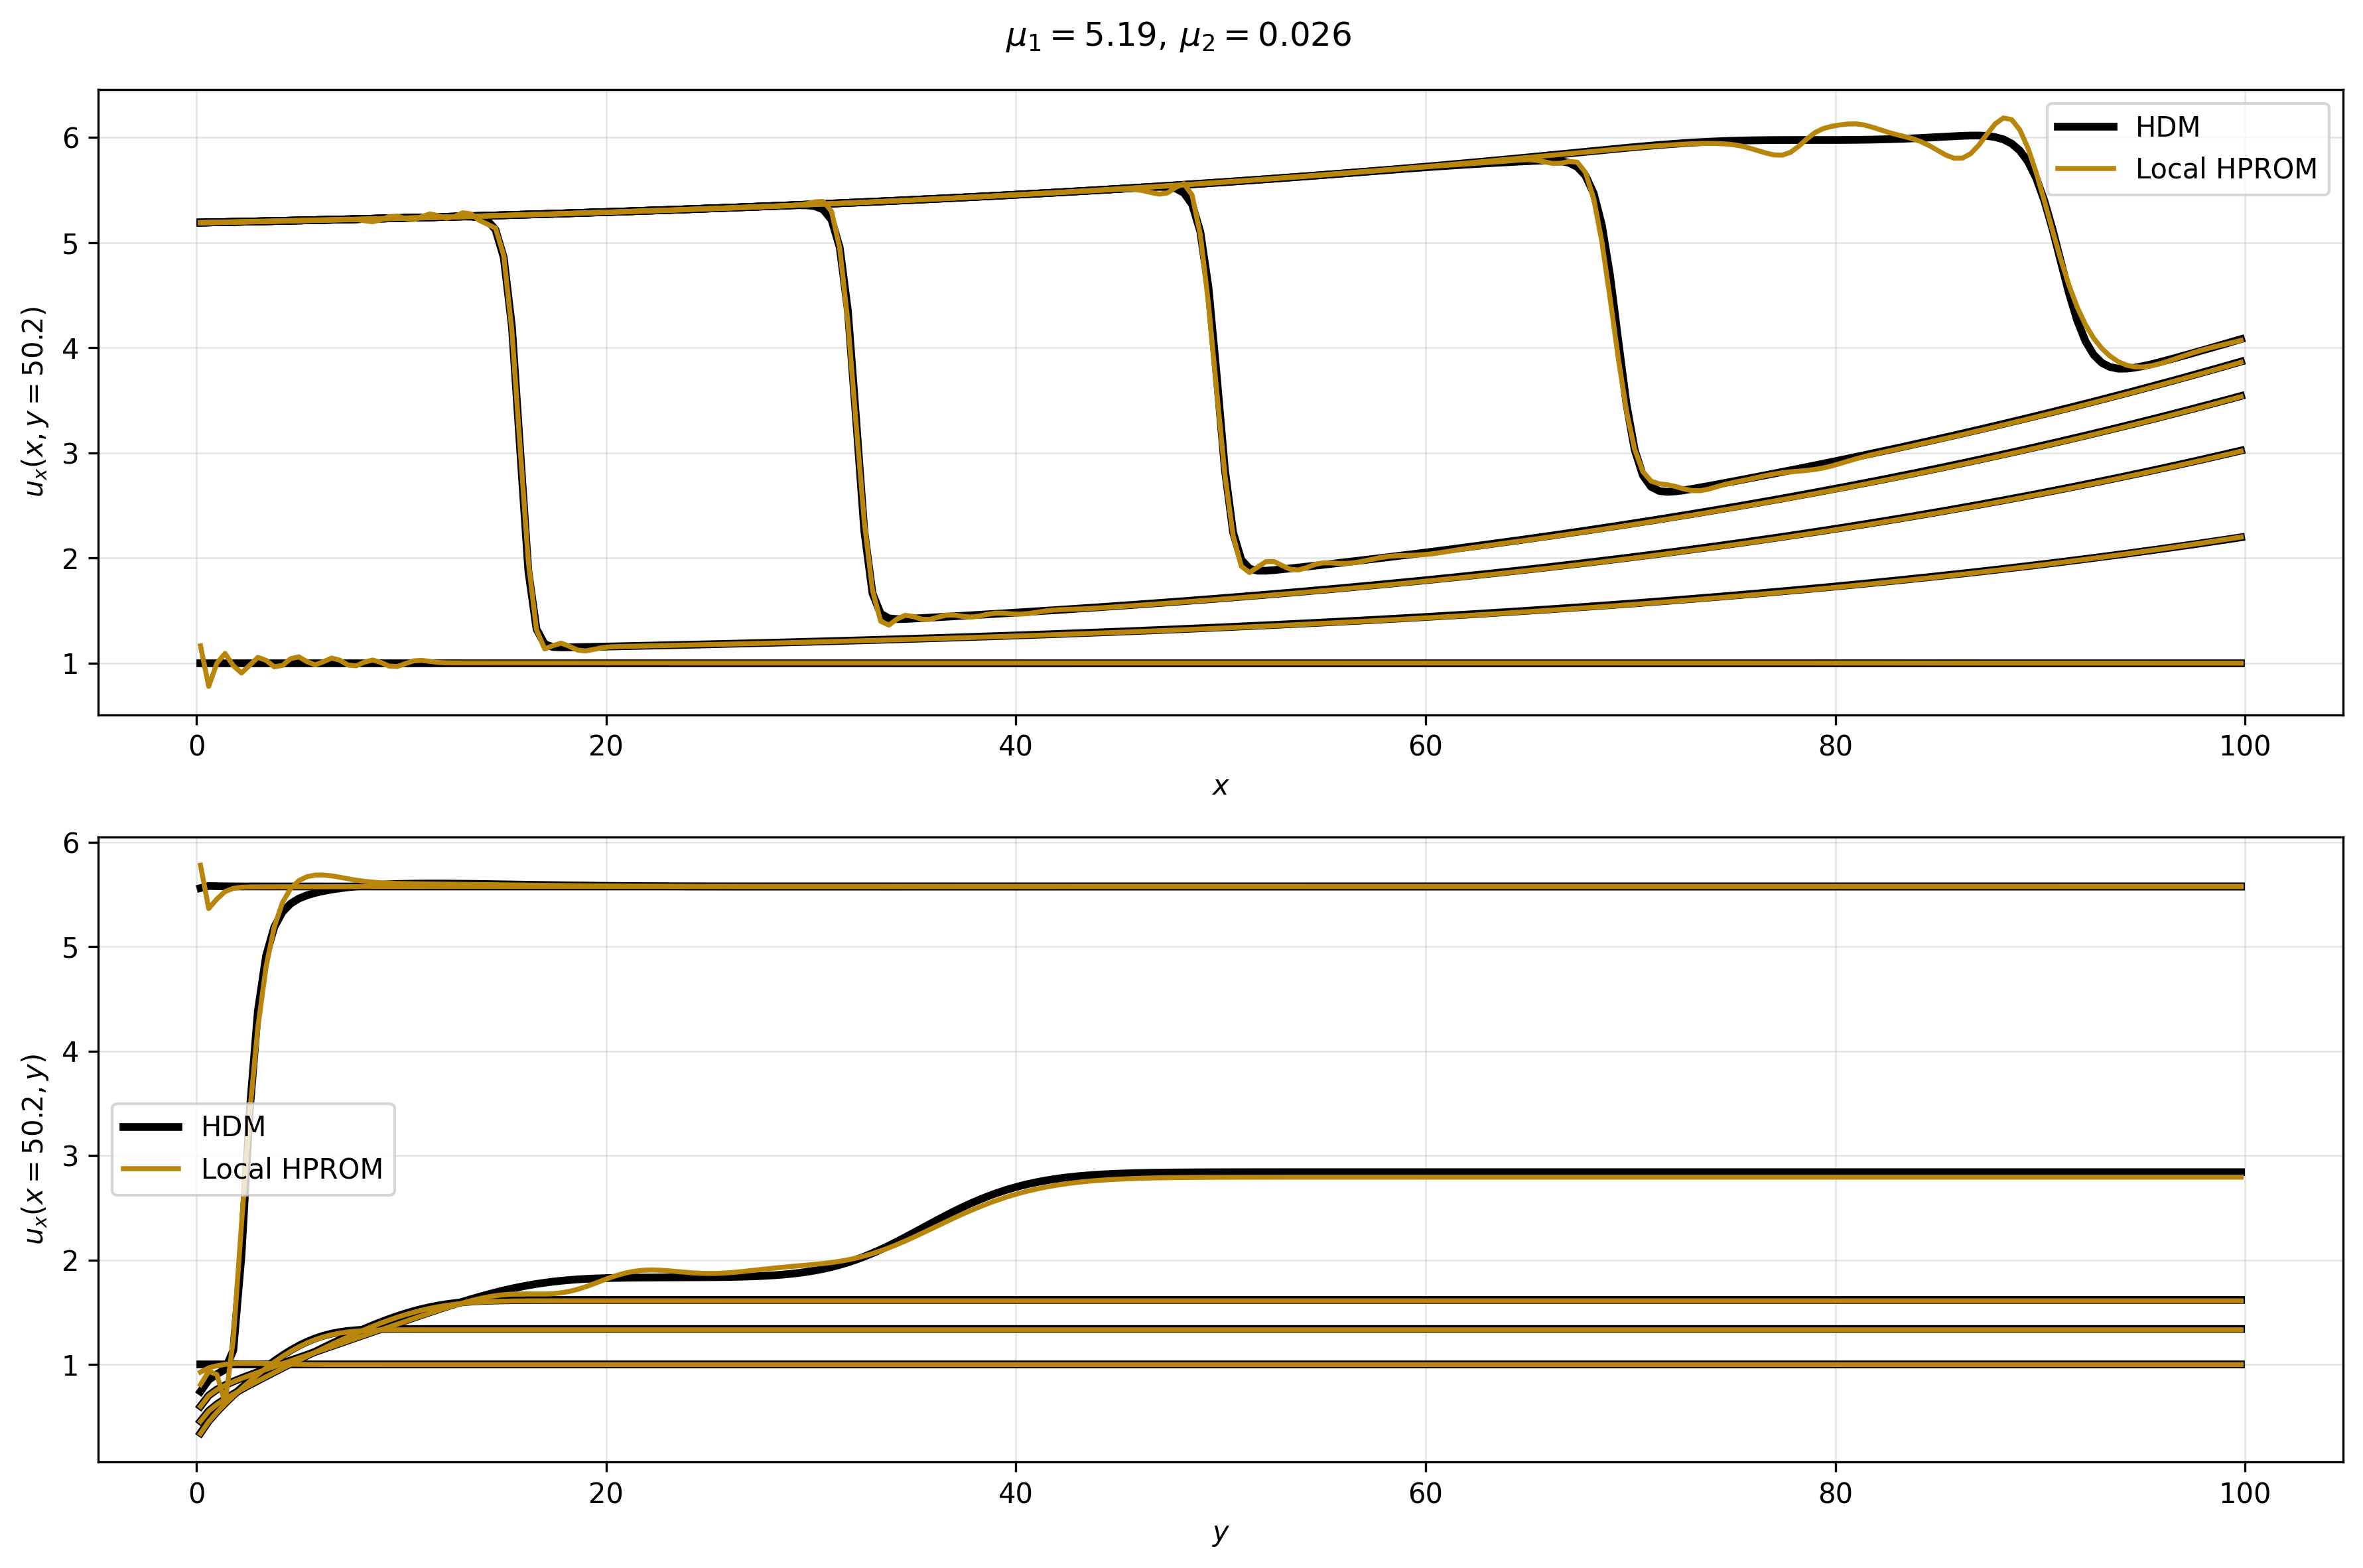
\includegraphics[width=0.82\textwidth,height=0.70\textheight,keepaspectratio]{Figures/local_hprom_vs_hdm_mu1_5.19_mu2_0.026_nc10.png}
\end{frame}

\begin{frame}{Appendix: Local HQPROM ($N_c=10$) vs HDM: $\boldsymbol\mu=(4.56,\,0.019)$}
\centering
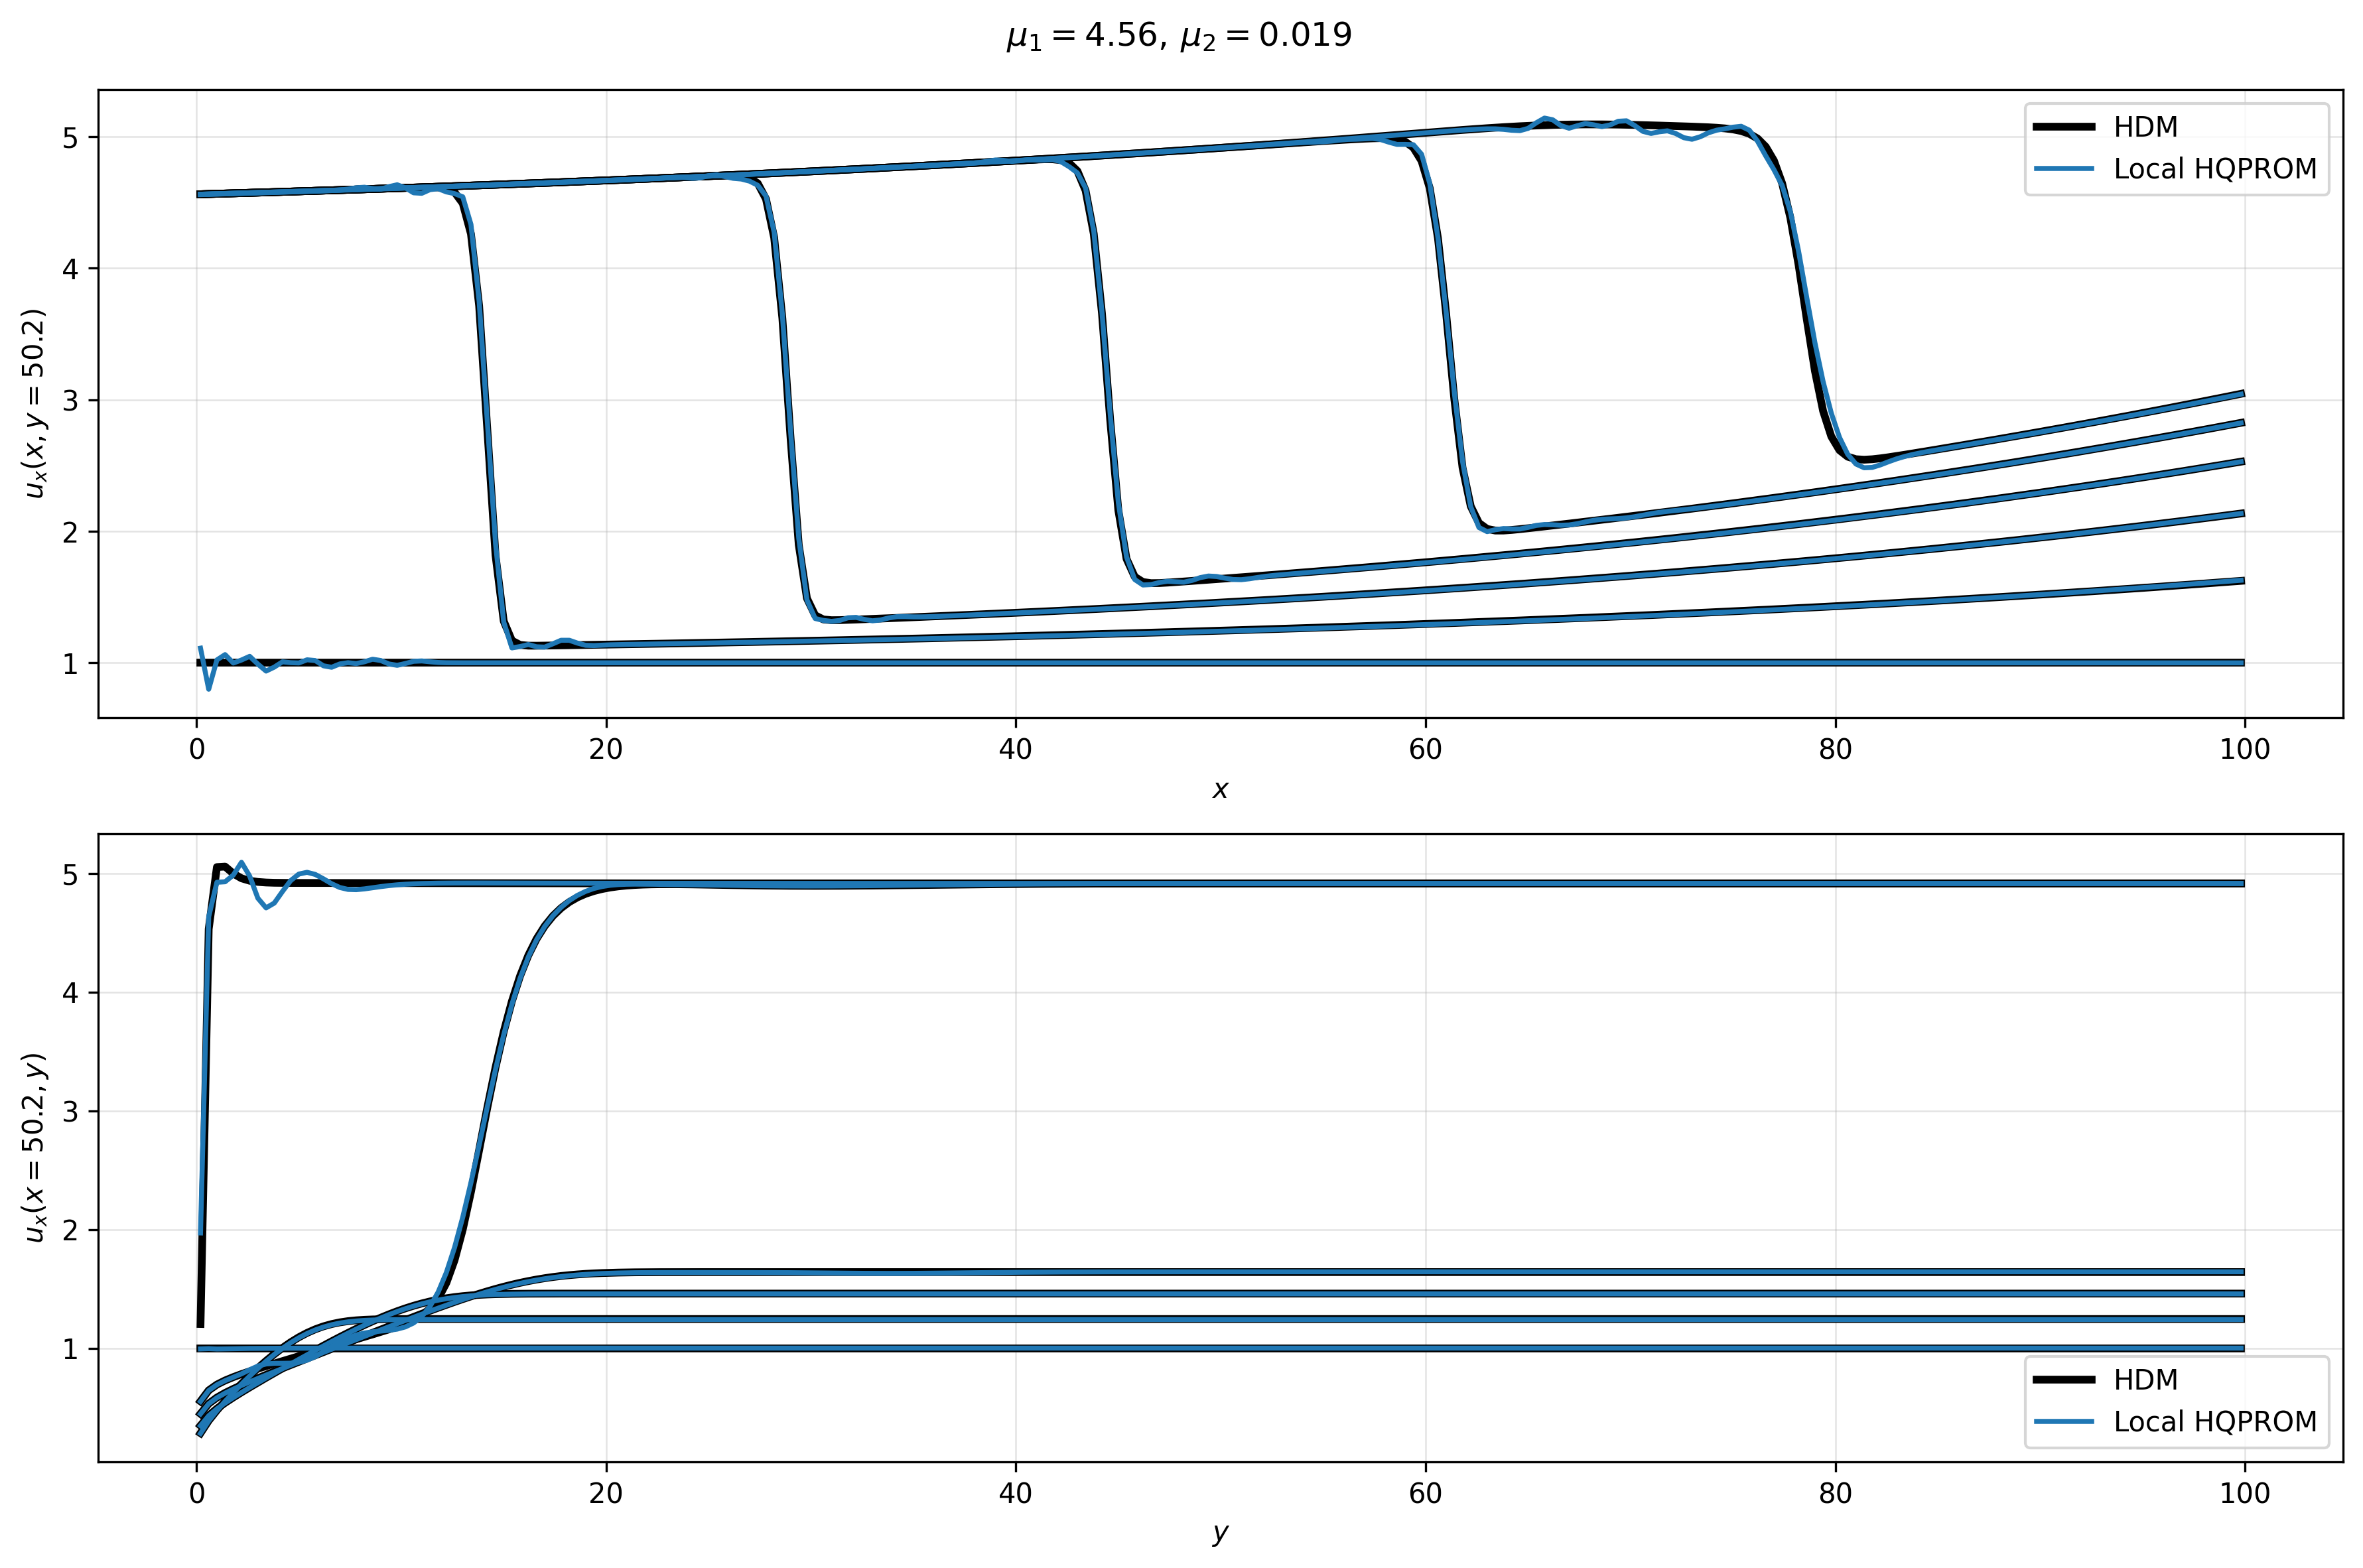
\includegraphics[width=0.82\textwidth,height=0.70\textheight,keepaspectratio]{Figures/local_hqprom_vs_hdm_mu1_4.56_mu2_0.019_nc10.png}
\end{frame}

\begin{frame}{Appendix: Local HQPROM ($N_c=10$) vs HDM: $\boldsymbol\mu=(4.75,\,0.020)$}
\centering
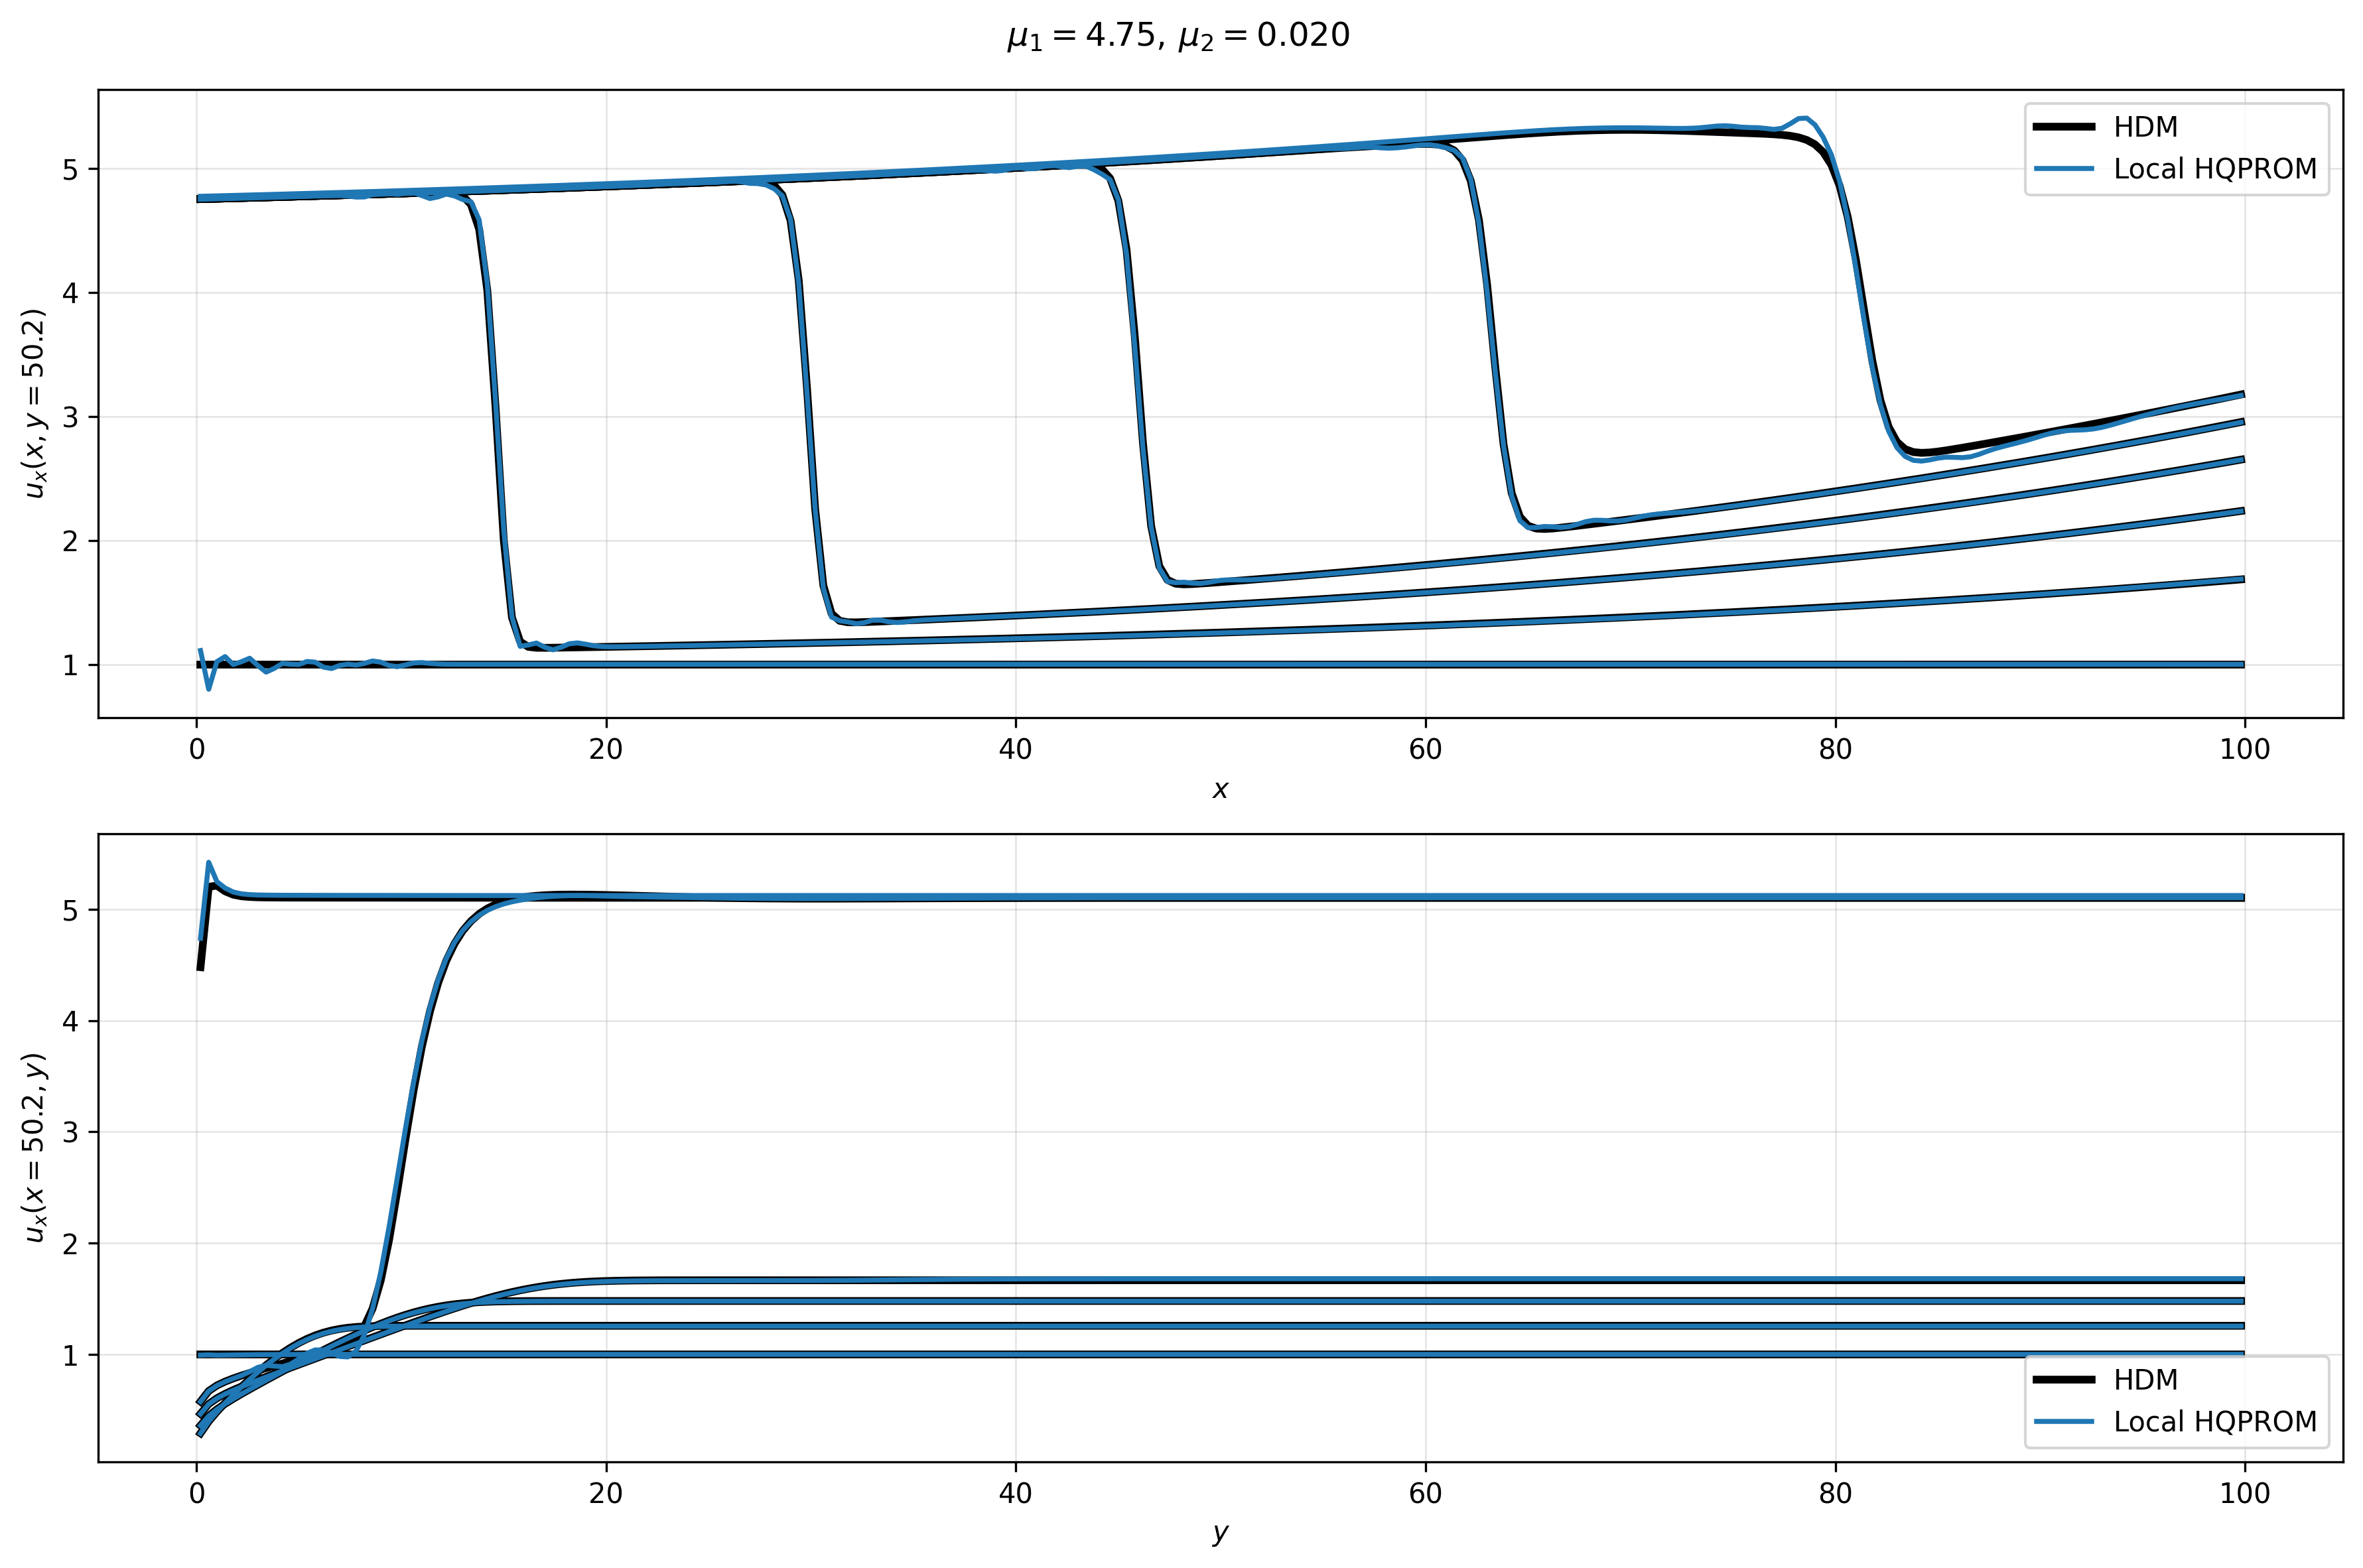
\includegraphics[width=0.82\textwidth,height=0.70\textheight,keepaspectratio]{Figures/local_hqprom_vs_hdm_mu1_4.75_mu2_0.020_nc10.png}
\end{frame}

\begin{frame}{Appendix: Local HQPROM ($N_c=10$) vs HDM: $\boldsymbol\mu=(5.19,\,0.026)$}
\centering
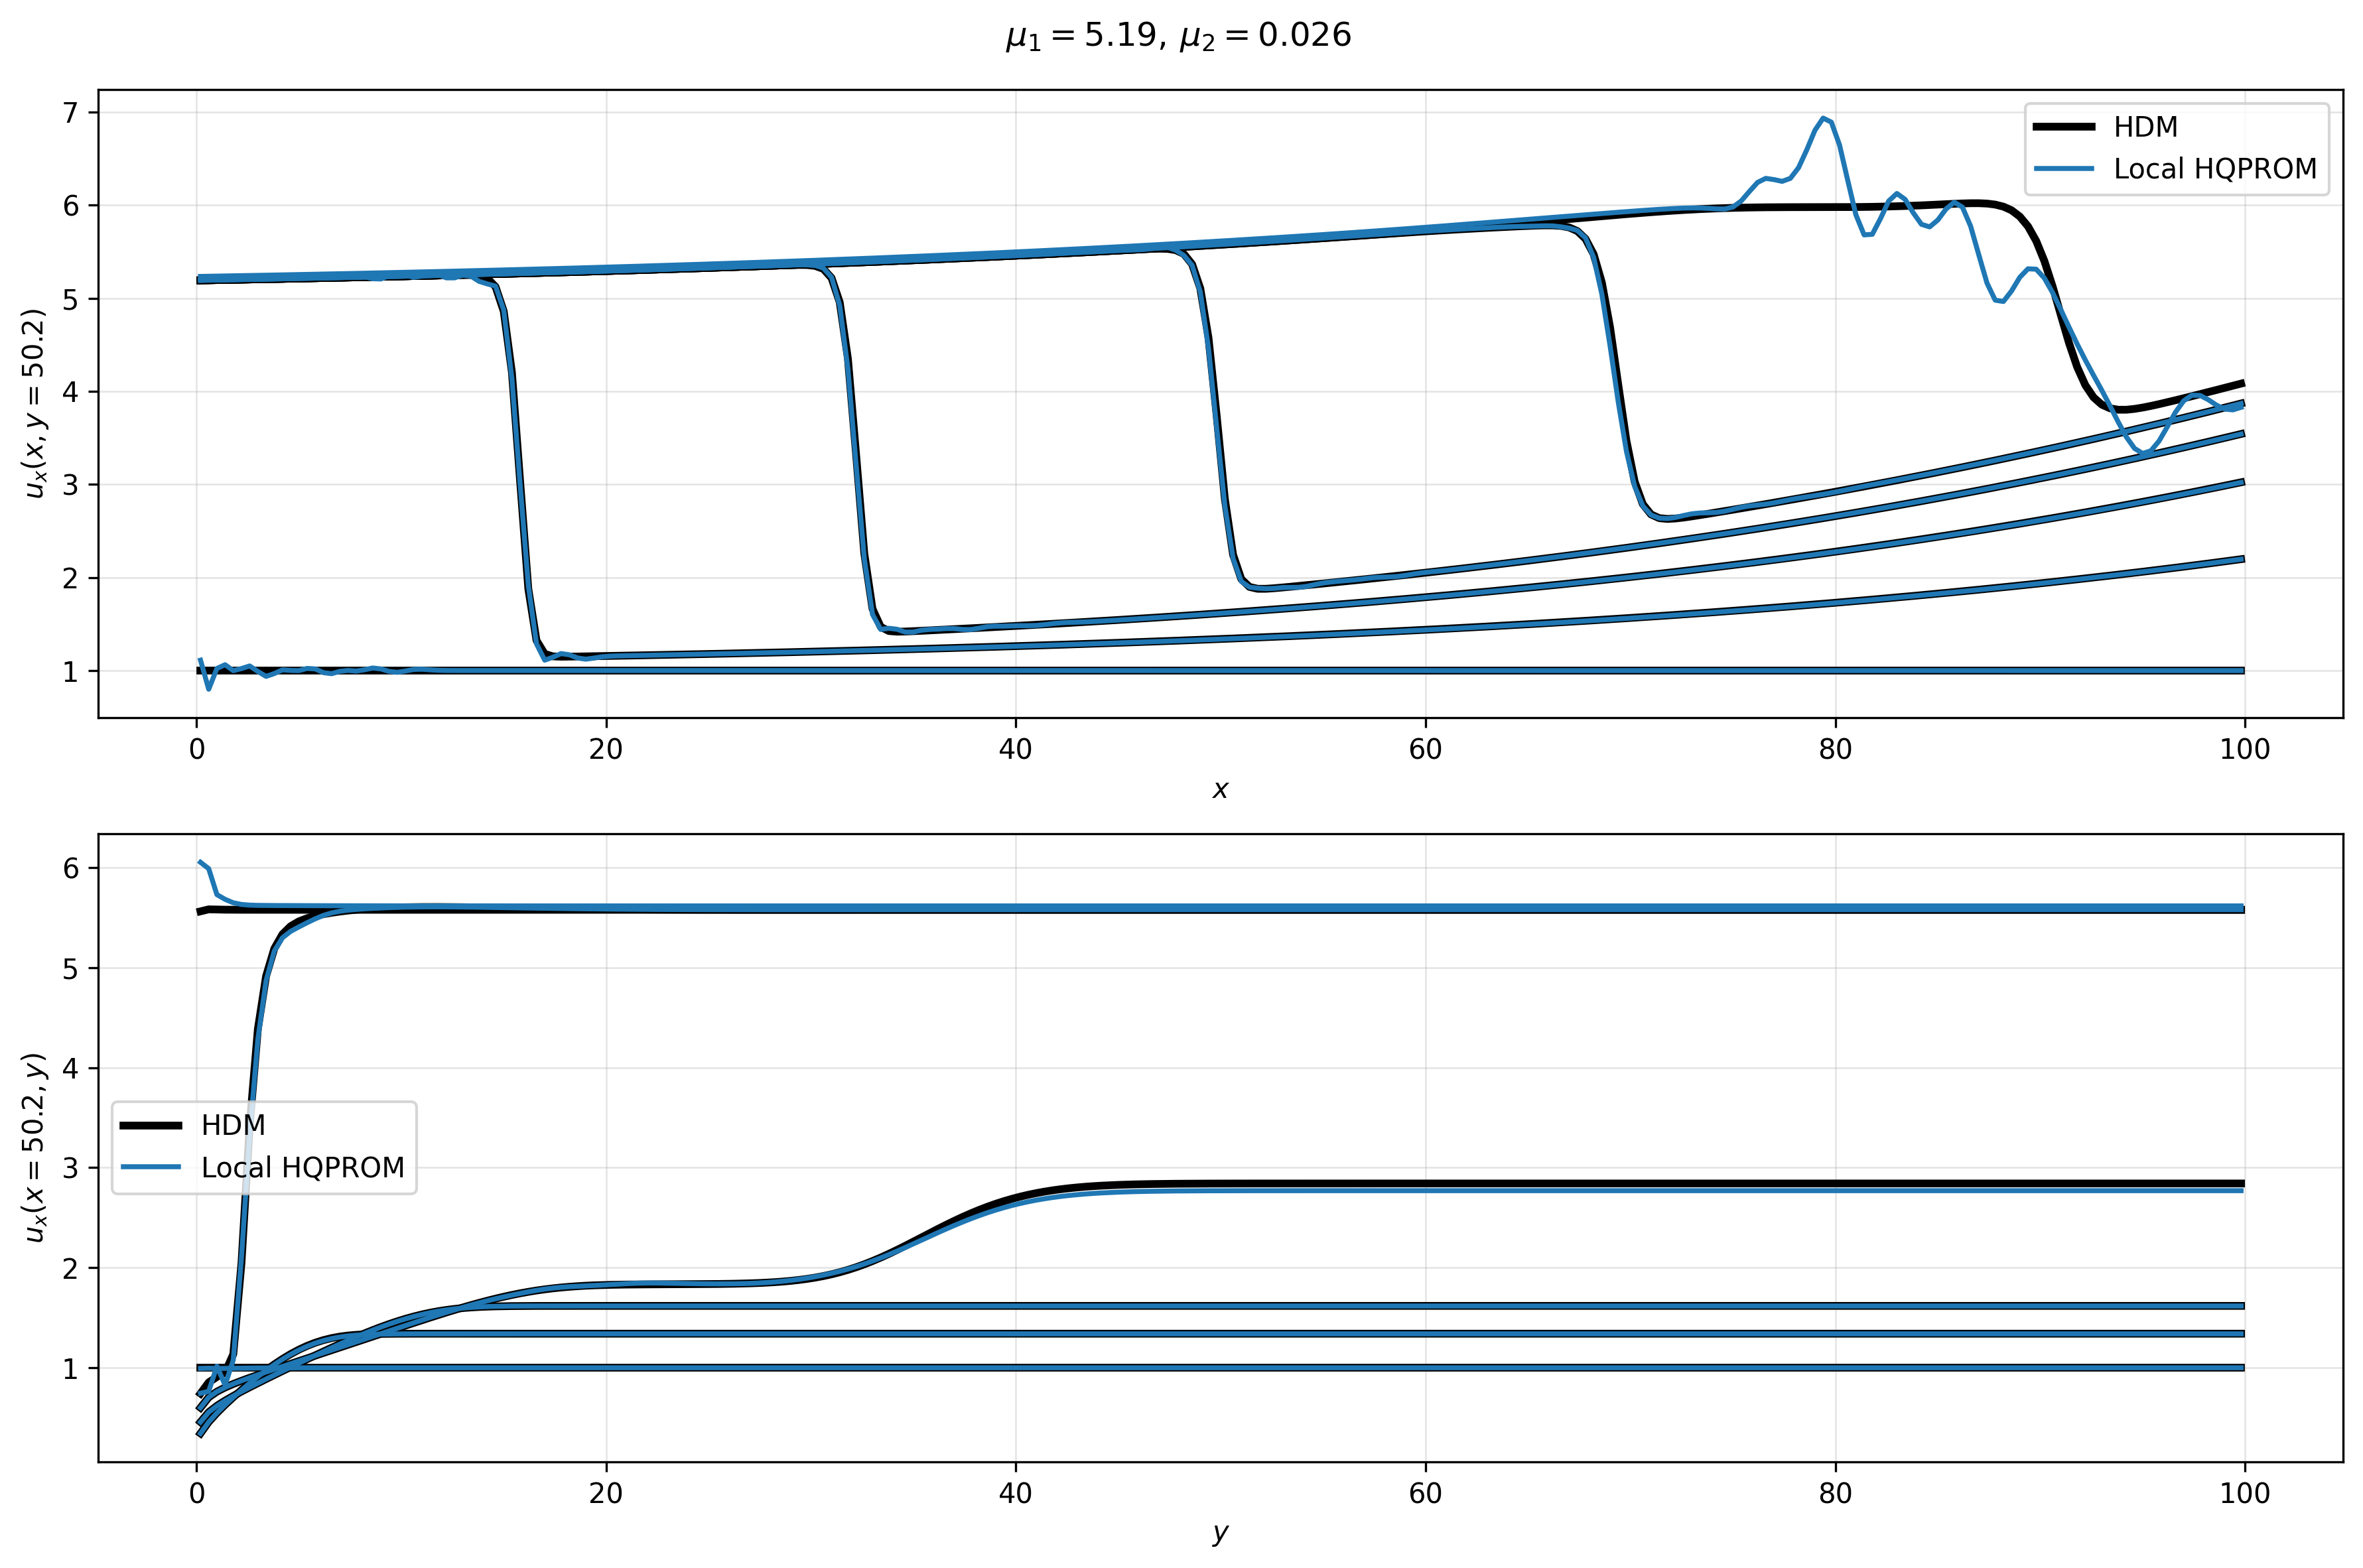
\includegraphics[width=0.82\textwidth,height=0.70\textheight,keepaspectratio]{Figures/local_hqprom_vs_hdm_mu1_5.19_mu2_0.026_nc10.png}
\end{frame}

\begin{frame}{Appendix: Local HPROM-GPR ($N_c=10$) vs HDM: $\boldsymbol\mu=(4.56,\,0.019)$}
\centering
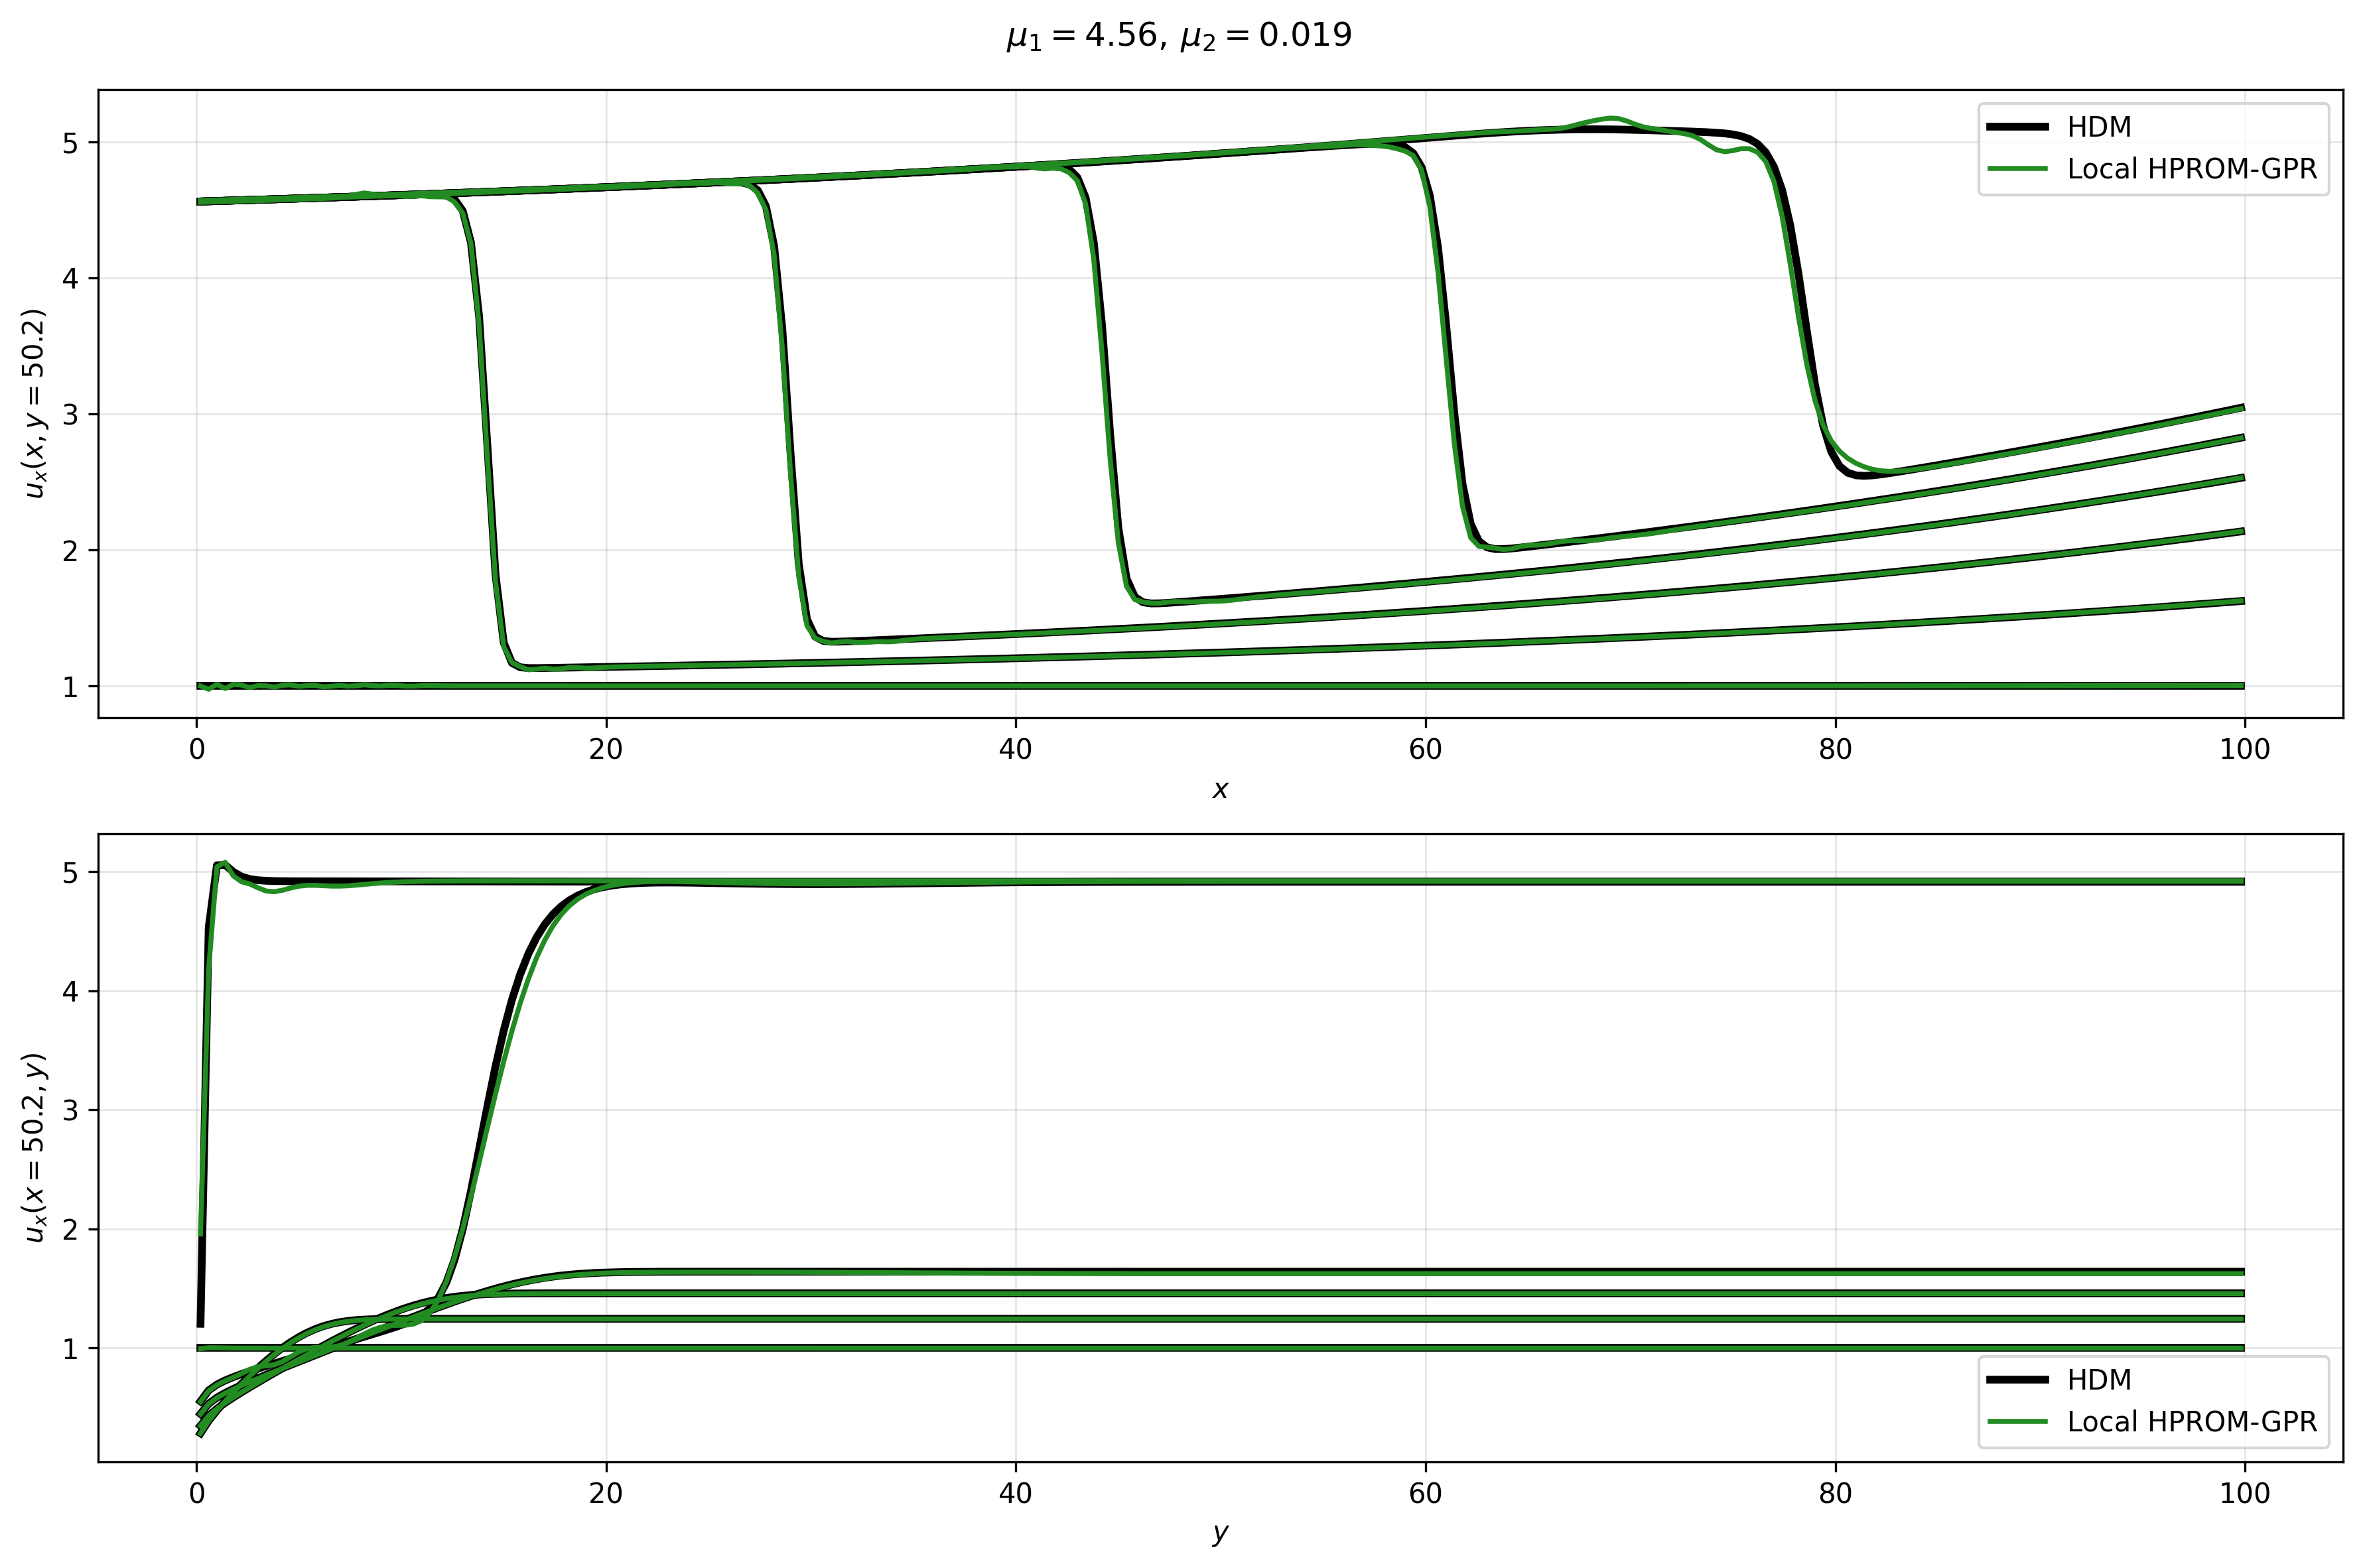
\includegraphics[width=0.82\textwidth,height=0.70\textheight,keepaspectratio]{Figures/local_hprom_gpr_vs_hdm_mu1_4.56_mu2_0.019_nc10.png}
\end{frame}

\begin{frame}{Appendix: Local HPROM-GPR ($N_c=10$) vs HDM: $\boldsymbol\mu=(4.75,\,0.020)$}
\centering
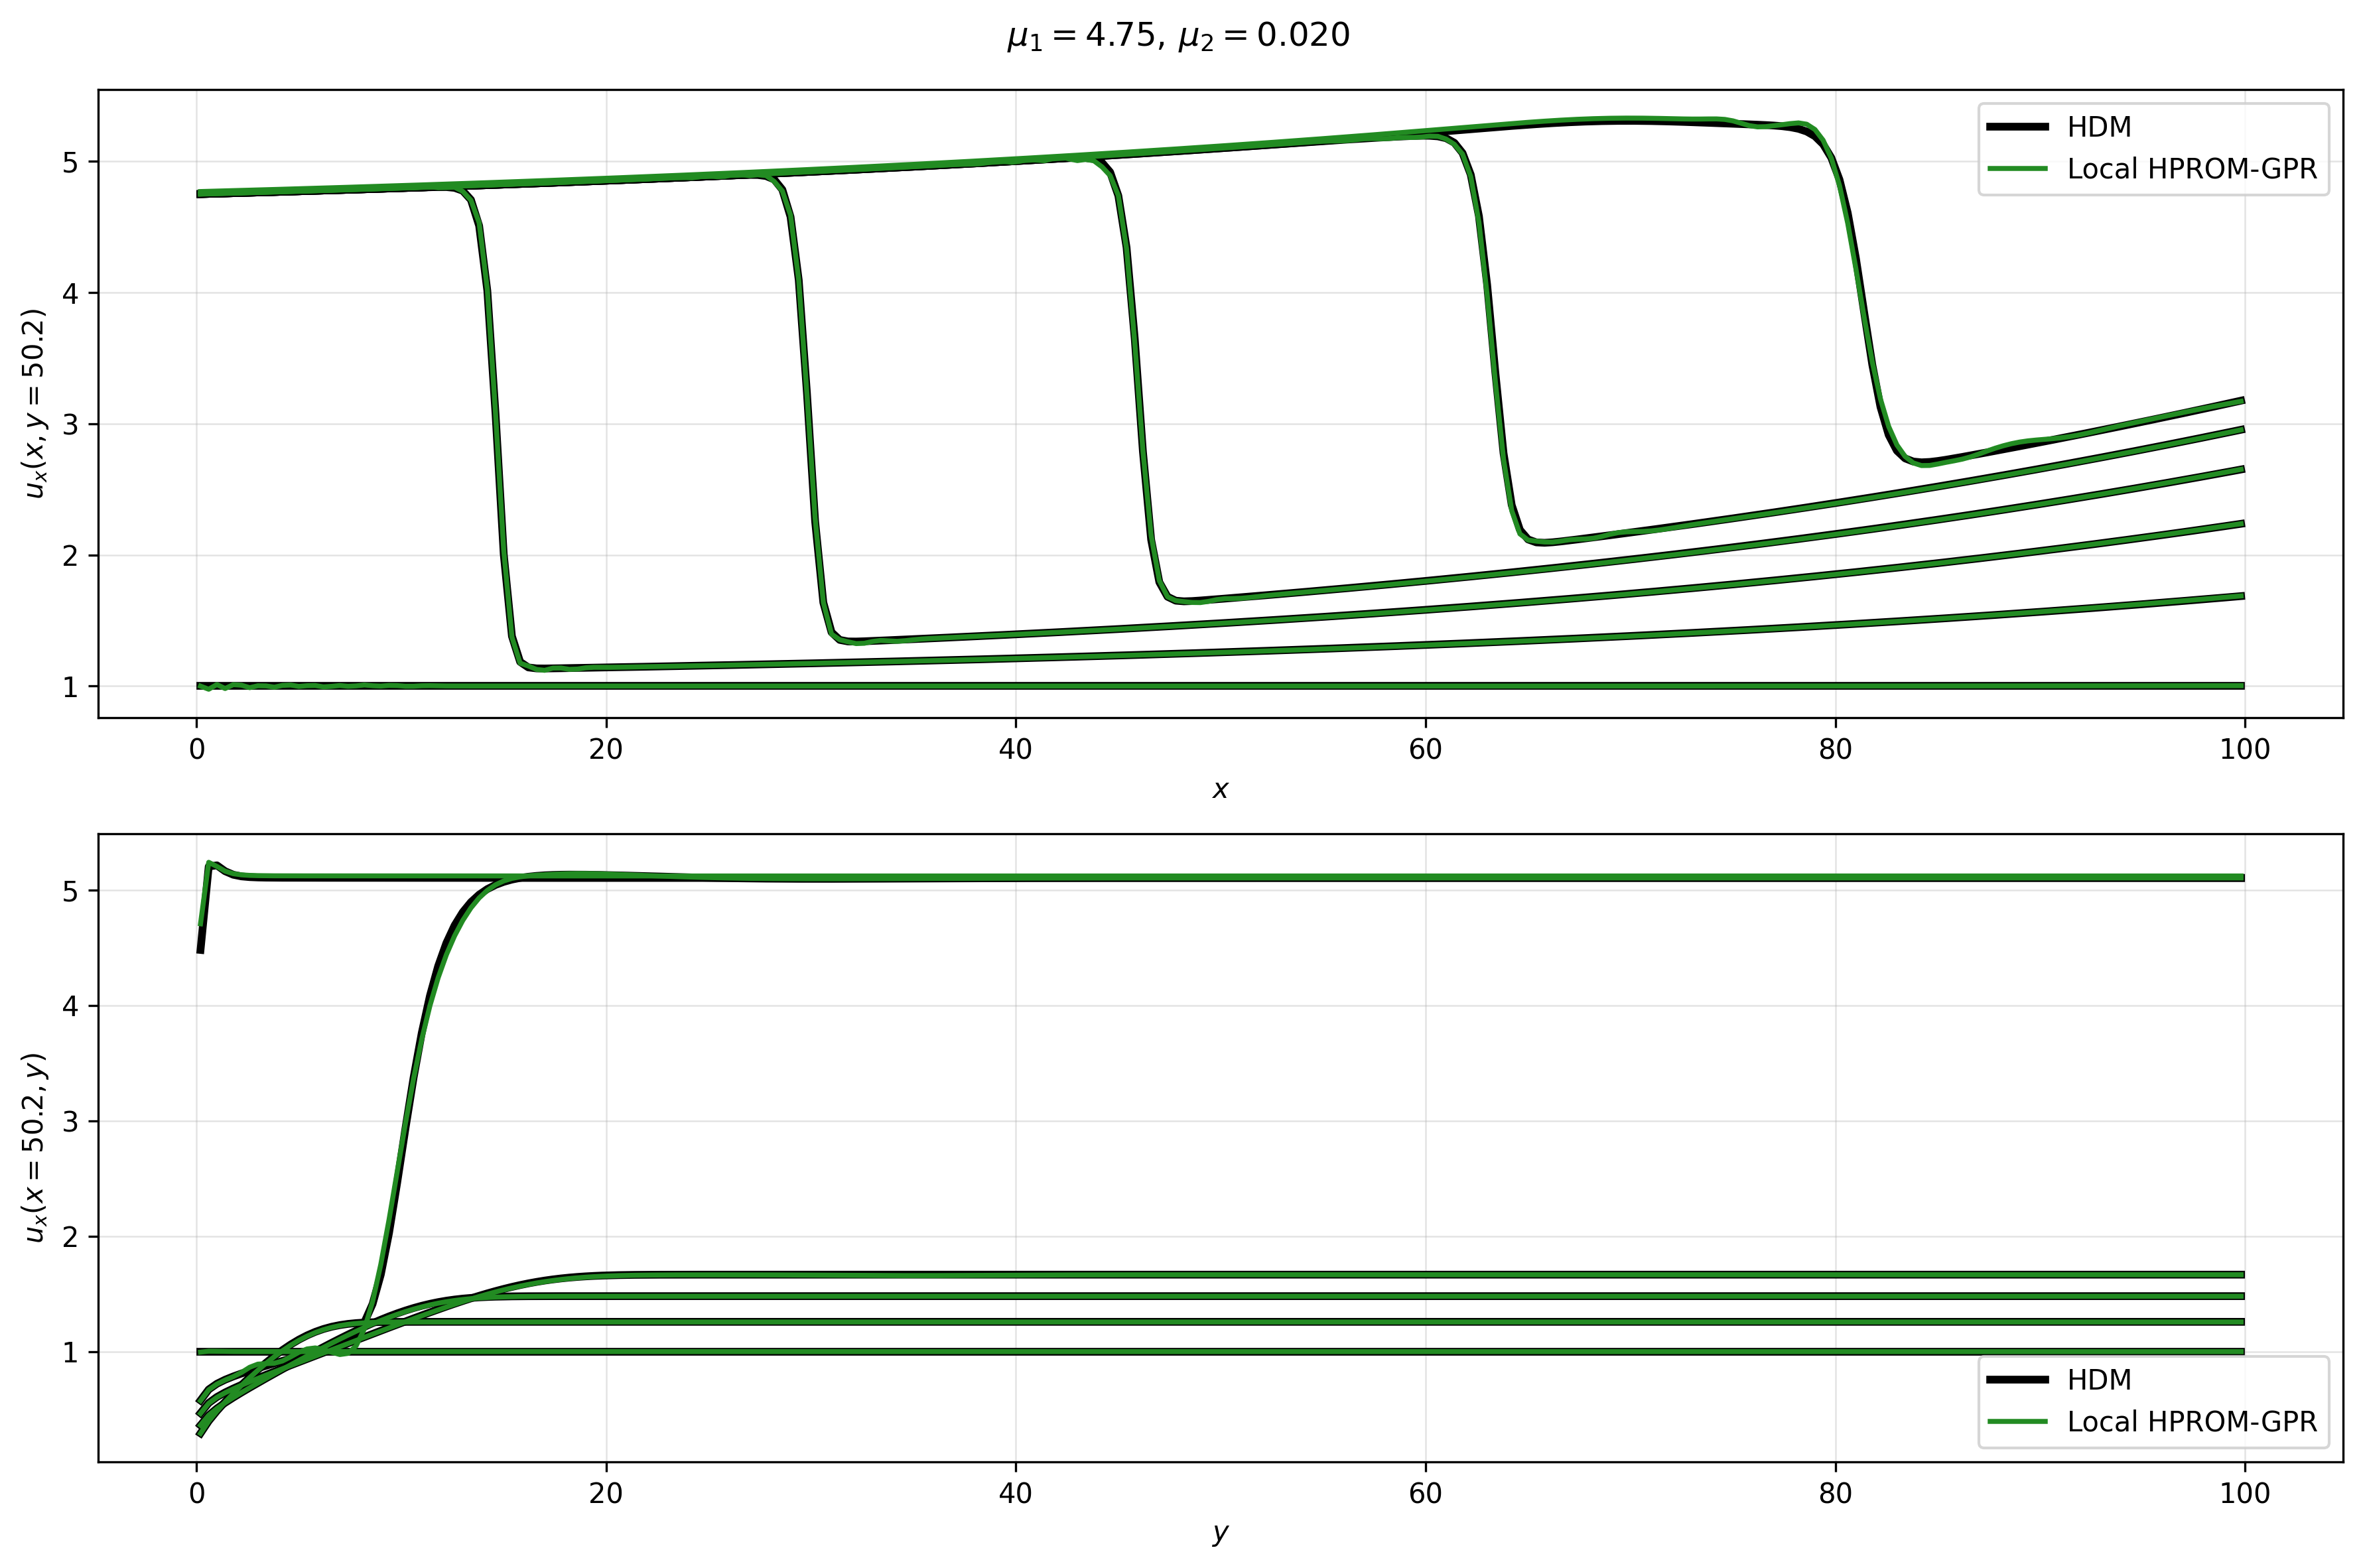
\includegraphics[width=0.82\textwidth,height=0.70\textheight,keepaspectratio]{Figures/local_hprom_gpr_vs_hdm_mu1_4.75_mu2_0.020_nc10.png}
\end{frame}

\begin{frame}{Appendix: Local HPROM-GPR ($N_c=10$) vs HDM: $\boldsymbol\mu=(5.19,\,0.026)$}
\centering
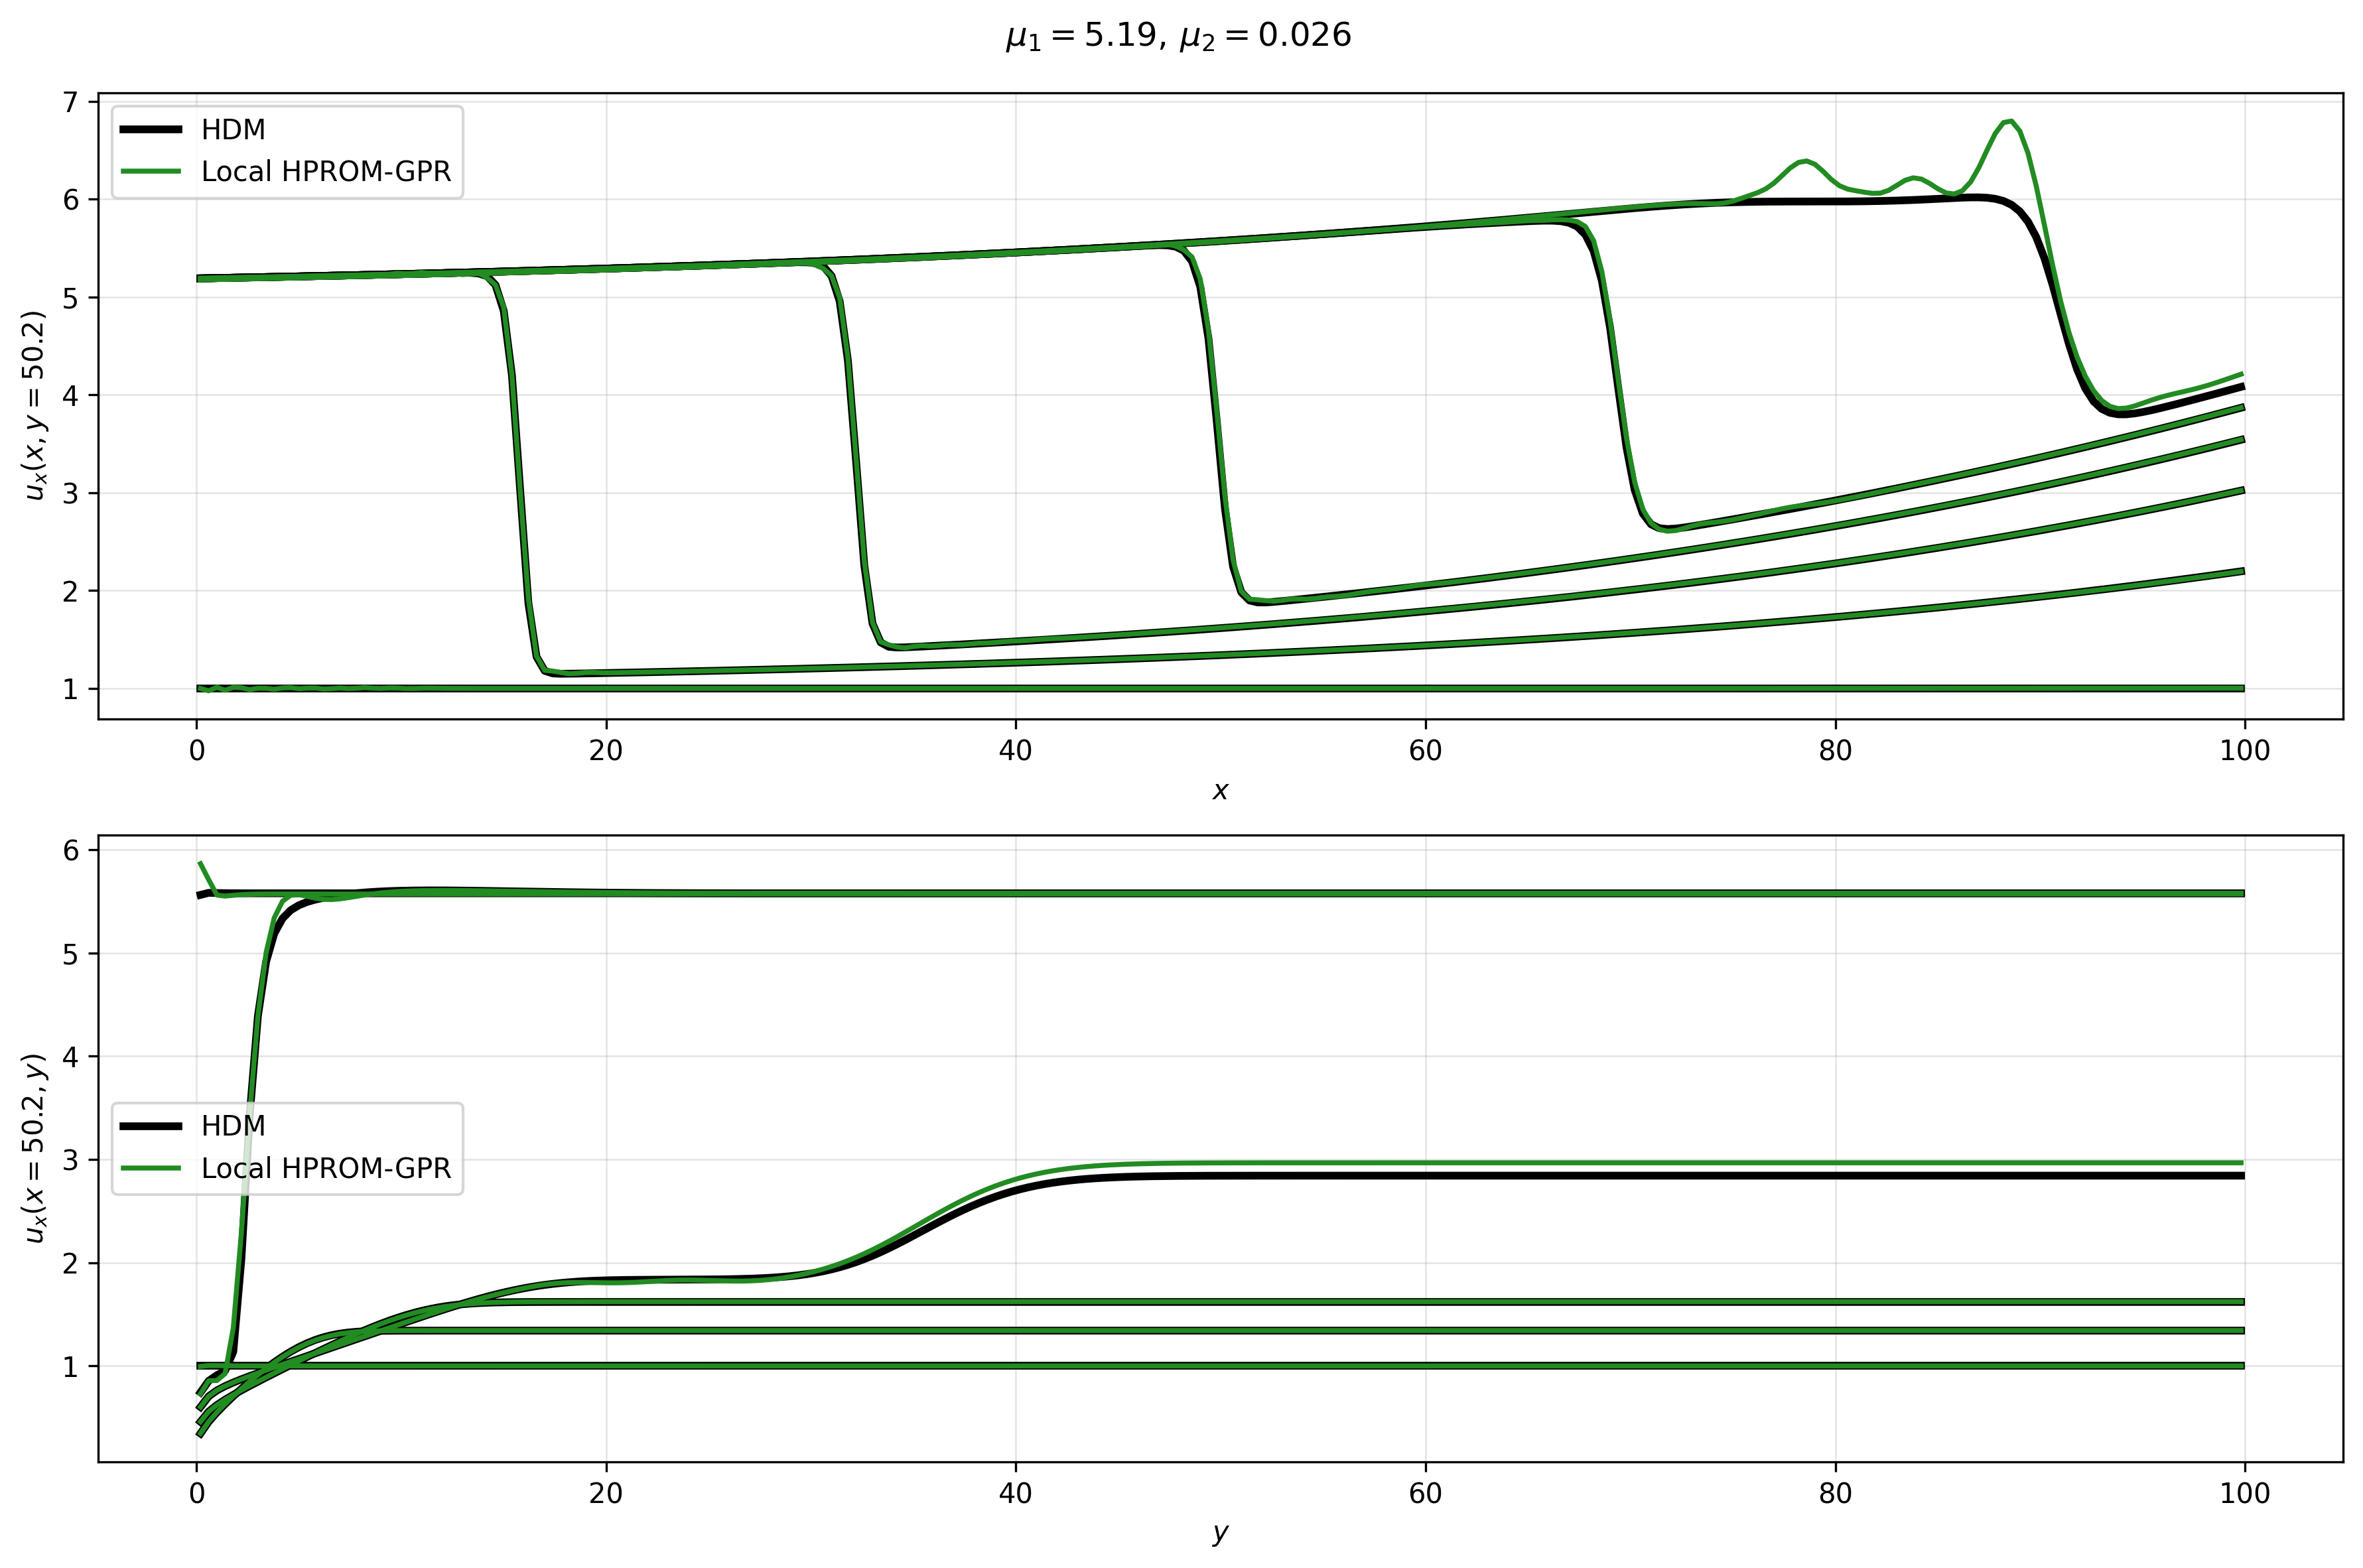
\includegraphics[width=0.82\textwidth,height=0.70\textheight,keepaspectratio]{Figures/local_hprom_gpr_vs_hdm_mu1_5.19_mu2_0.026_nc10.png}
\end{frame}

\begin{frame}{Appendix: Linear Selector Expansion}
\scriptsize
\[
\mathbf u^s=\mathbf u_{0,k^-}+\mathbf V_{k^-}\mathbf q_{k^-},
\qquad
k^+=\arg\min_{\ell}\|\mathbf u^s-\mathbf u_{c,\ell}\|_2^2.
\]
\[
\text{Let }\mathbf a_\ell:=\mathbf u_{0,k^-}-\mathbf u_{c,\ell},\quad
\mathbf b:=\mathbf V_{k^-}\mathbf q_{k^-}.
\]
\[
\|\mathbf u^s-\mathbf u_{c,\ell}\|_2^2
=\|\mathbf a_\ell+\mathbf b\|_2^2
=\|\mathbf a_\ell\|_2^2+\|\mathbf b\|_2^2+2\,\mathbf a_\ell^T\mathbf b.
\]
\[
\|\mathbf b\|_2^2=\|\mathbf V_{k^-}\mathbf q_{k^-}\|_2^2
\ \text{is independent of }\ell.
\]
\[
\Rightarrow\
k^+=\arg\min_{\ell}
\Big[
\|\mathbf u_{0,k^-}-\mathbf u_{c,\ell}\|_2^2
+2(\mathbf u_{0,k^-}-\mathbf u_{c,\ell})^T\mathbf V_{k^-}\mathbf q_{k^-}
\Big].
\]
Precompute
\[
\mathbf g_{k^-,\ell}:=\mathbf V_{k^-}^T(\mathbf u_{0,k^-}-\mathbf u_{c,\ell}),
\qquad
d_{k^-,\ell}:=\|\mathbf u_{0,k^-}-\mathbf u_{c,\ell}\|_2^2,
\]
which yields
\[
k^+=\arg\min_{\ell}\left(2\,\mathbf g_{k^-,\ell}^T\mathbf q_{k^-}+d_{k^-,\ell}\right).
\]
\end{frame}

\begin{frame}{Appendix: HQPROM Selector Expansion}
\scriptsize
\[
\mathbf u^s=\mathbf u_{0,k^-}+\mathbf V_{k^-}\mathbf q_{k^-}
+\mathbf H_{k^-}(\mathbf q_{k^-}\otimes\mathbf q_{k^-}).
\]
\[
\text{Let }\mathbf a_\ell:=\mathbf u_{0,k^-}-\mathbf u_{c,\ell},\quad
\mathbf b:=\mathbf V_{k^-}\mathbf q_{k^-},\quad
\mathbf c:=\mathbf H_{k^-}(\mathbf q_{k^-}\otimes\mathbf q_{k^-}).
\]
\[
k^+=\arg\min_{\ell}\|\mathbf u^s-\mathbf u_{c,\ell}\|_2^2
=
\arg\min_{\ell}
\|\mathbf a_\ell+\mathbf b+\mathbf c\|_2^2.
\]
\[
\|\mathbf a_\ell+\mathbf b+\mathbf c\|_2^2
=\|\mathbf a_\ell\|_2^2+\|\mathbf b\|_2^2+\|\mathbf c\|_2^2
+2\,\mathbf a_\ell^T\mathbf b
+2\,\mathbf a_\ell^T\mathbf c
+2\,\mathbf b^T\mathbf c.
\]
\[
\|\mathbf b\|_2^2,\ \|\mathbf c\|_2^2,\ 2\,\mathbf b^T\mathbf c
\ \text{are independent of }\ell.
\]
\[
\Rightarrow\
k^+=\arg\min_{\ell}
\Big[
\|\mathbf u_{0,k^-}-\mathbf u_{c,\ell}\|_2^2
\]
\[
\quad
+2(\mathbf u_{0,k^-}-\mathbf u_{c,\ell})^T\mathbf V_{k^-}\mathbf q_{k^-}
+2(\mathbf u_{0,k^-}-\mathbf u_{c,\ell})^T\mathbf H_{k^-}(\mathbf q_{k^-}\otimes\mathbf q_{k^-})
\Big].
\]
Define
\[
\mathbf m_{k^-,\ell}^T(\mathbf q\otimes\mathbf q)
:=
(\mathbf u_{0,k^-}-\mathbf u_{c,\ell})^T\mathbf H_{k^-}(\mathbf q\otimes\mathbf q),
\]
then
\[
k^+=\arg\min_{\ell}
\left(
2\,\mathbf g_{k^-,\ell}^T\mathbf q_{k^-}
+2\,\mathbf m_{k^-,\ell}^T(\mathbf q_{k^-}\otimes\mathbf q_{k^-})
+d_{k^-,\ell}
\right).
\]
\end{frame}

\begin{frame}{Appendix: HPROM-GPR Selector Expansion}
\scriptsize
\[
\mathbf u^s=
\mathbf u_{0,k^-}
+\mathbf V_{k^-}\mathbf q_{k^-}
+\bar{\mathbf V}_{k^-}\bar{\mathbf q}_{k^-},
\qquad
\bar{\mathbf q}_{k^-}=\mathcal N_{\mathrm{GPR},k^-}(\mathbf q_{k^-}).
\]
\[
\text{Let }\mathbf a_\ell:=\mathbf u_{0,k^-}-\mathbf u_{c,\ell},\quad
\mathbf b:=\mathbf V_{k^-}\mathbf q_{k^-},\quad
\mathbf c:=\bar{\mathbf V}_{k^-}\bar{\mathbf q}_{k^-}.
\]
\[
\|\mathbf u^s-\mathbf u_{c,\ell}\|_2^2
=\|\mathbf a_\ell+\mathbf b+\mathbf c\|_2^2
\]
\[
\ =\ \|\mathbf a_\ell\|_2^2+\|\mathbf b\|_2^2+\|\mathbf c\|_2^2
+2\,\mathbf a_\ell^T\mathbf b
+2\,\mathbf a_\ell^T\mathbf c
+2\,\mathbf b^T\mathbf c.
\]
\[
\|\mathbf b\|_2^2,\ \|\mathbf c\|_2^2,\ 2\,\mathbf b^T\mathbf c
\ \text{are independent of }\ell.
\]
\[
\Rightarrow\
k^+=\arg\min_{\ell}
\Big[
\|\mathbf u_{0,k^-}-\mathbf u_{c,\ell}\|_2^2
+2(\mathbf u_{0,k^-}-\mathbf u_{c,\ell})^T\mathbf V_{k^-}\mathbf q_{k^-}
+2(\mathbf u_{0,k^-}-\mathbf u_{c,\ell})^T\bar{\mathbf V}_{k^-}\bar{\mathbf q}_{k^-}
\Big].
\]
Hence, with
\[
\bar{\mathbf g}_{k^-,\ell}:=\bar{\mathbf V}_{k^-}^T(\mathbf u_{0,k^-}-\mathbf u_{c,\ell}),
\]
\[
k^+=\arg\min_{\ell}
\left(
2\,\mathbf g_{k^-,\ell}^T\mathbf q_{k^-}
+2\,\bar{\mathbf g}_{k^-,\ell}^T\bar{\mathbf q}_{k^-}
+d_{k^-,\ell}
\right).
\]
\end{frame}

\end{document}
